\documentclass[twoside,12pt]{article}
\usepackage[a4paper, margin=2.5cm]{geometry}


%PDFLatex obsolete packages:
%	\usepackage[utf8]{inputenc}
%	\usepackage[T1]{fontenc}
%	\usepackage[polish]{babel}
%	\usepackage{lmodern}

%LuaTex packages:
	\usepackage{fontspec}
	\setmainfont{Times New Roman}\let\emph\textit
	\usepackage{polski}
	\defaultfontfeatures{Ligatures=TeX} %ligatury w luatex

%tekst:
	\usepackage{setspace} \onehalfspacing %interlinie 1.5
	%\usepackage{indentfirst} %aby pierwszy paragraf również był wcięty
	%\usepackage[ampersand]{easylist} %łatwiejsze listy
	\usepackage{verbatim} %środowisko kodu
	\usepackage{microtype} %poprawki tekstu
	%\usepackage{titlesec} %tytuły sekcji i rozdziałów
	\usepackage{textcomp} %symbole text companion

%tabele:
	\usepackage{hhline} %linie poziome w tabelach
	\usepackage{tabu}
	\usepackage{booktabs}
	\usepackage{bigstrut}
	\usepackage{multirow}

%nagłówki:
	\usepackage{fancyhdr} 

%matematyka
	\usepackage{amsmath} %zapis matematyczny
	\usepackage{amsfonts} %znaki matematyczne
	\usepackage{siunitx} %jednostki SI
	\usepackage{fp} %obliczenia zmiennoprzecinkowe
	\usepackage{gensymb} %symbole
	\usepackage{ifthen}

%figury:
	\usepackage{float} %aby użyć [H]
	\usepackage{pgfplots}	\pgfplotsset{width=10cm,compat=1.9} %obrazki z pdfów
	\usepackage{caption} \captionsetup{justification=centering,labelfont=bf} %podpisy pod obrazkami
	\usepackage{graphicx}	\graphicspath{ {img/} } %importowanie obrazów
	\usepackage{subcaption} %dodatkowe captions dla subfigur
	
%wdowy i sieroty
	%\widowpenalty=10000
	%\clubpenalty=10000

	\usepackage{hyperref} %odnosniki
	\hypersetup{colorlinks=true, linkcolor=black, filecolor=magenta, urlcolor=blue, citecolor=black}

\usepackage{pdfpages}


\title{Praca magisterska}
\author{Bartosz Surma}
\date{}

%------------------------------------------------------------------------------------------------------------------------------------------------
%HEADER

\pagestyle{fancy}

\fancyfoot{}
\fancyhead{}

\fancyhead[L]{Studia węzłów przesiadkowych \\ tramwaj – autobus – Park and Ride}
\fancyhead[R]{inż. Bartosz Surma}

\fancyfoot[RE,LO]{\thepage}
\renewcommand{\headrulewidth}{0.4pt}
\renewcommand{\footrulewidth}{0.4pt}
\setlength{\headsep}{1cm}


\pagestyle{fancy}

%------------------------------------------------------------------------------------------------------------------------------------------------
%DOCUMENT

%---------------------------------------------
\setlength{\parindent}{0em}
\setlength{\parskip}{0.5cm plus0.5cm minus0.5cm}
\raggedbottom
%---------------------------------------------

\begin{document}

%STYL PARAGRAFÓW:
%\titleformat{\section}{\normalfont\scshape}{\thesection}{16pt}{}
%\titleformat{\subsection}{\normalfont\scshape}{\thesubsection}{14pt}{}
%\titleformat{\subsubsection}{\normalfont\scshape}{\thesubsubsection}{12pt}{}

%STRONA TYTUŁOWA:
%\input{titlepage}
	%\pagestyle{empty}
	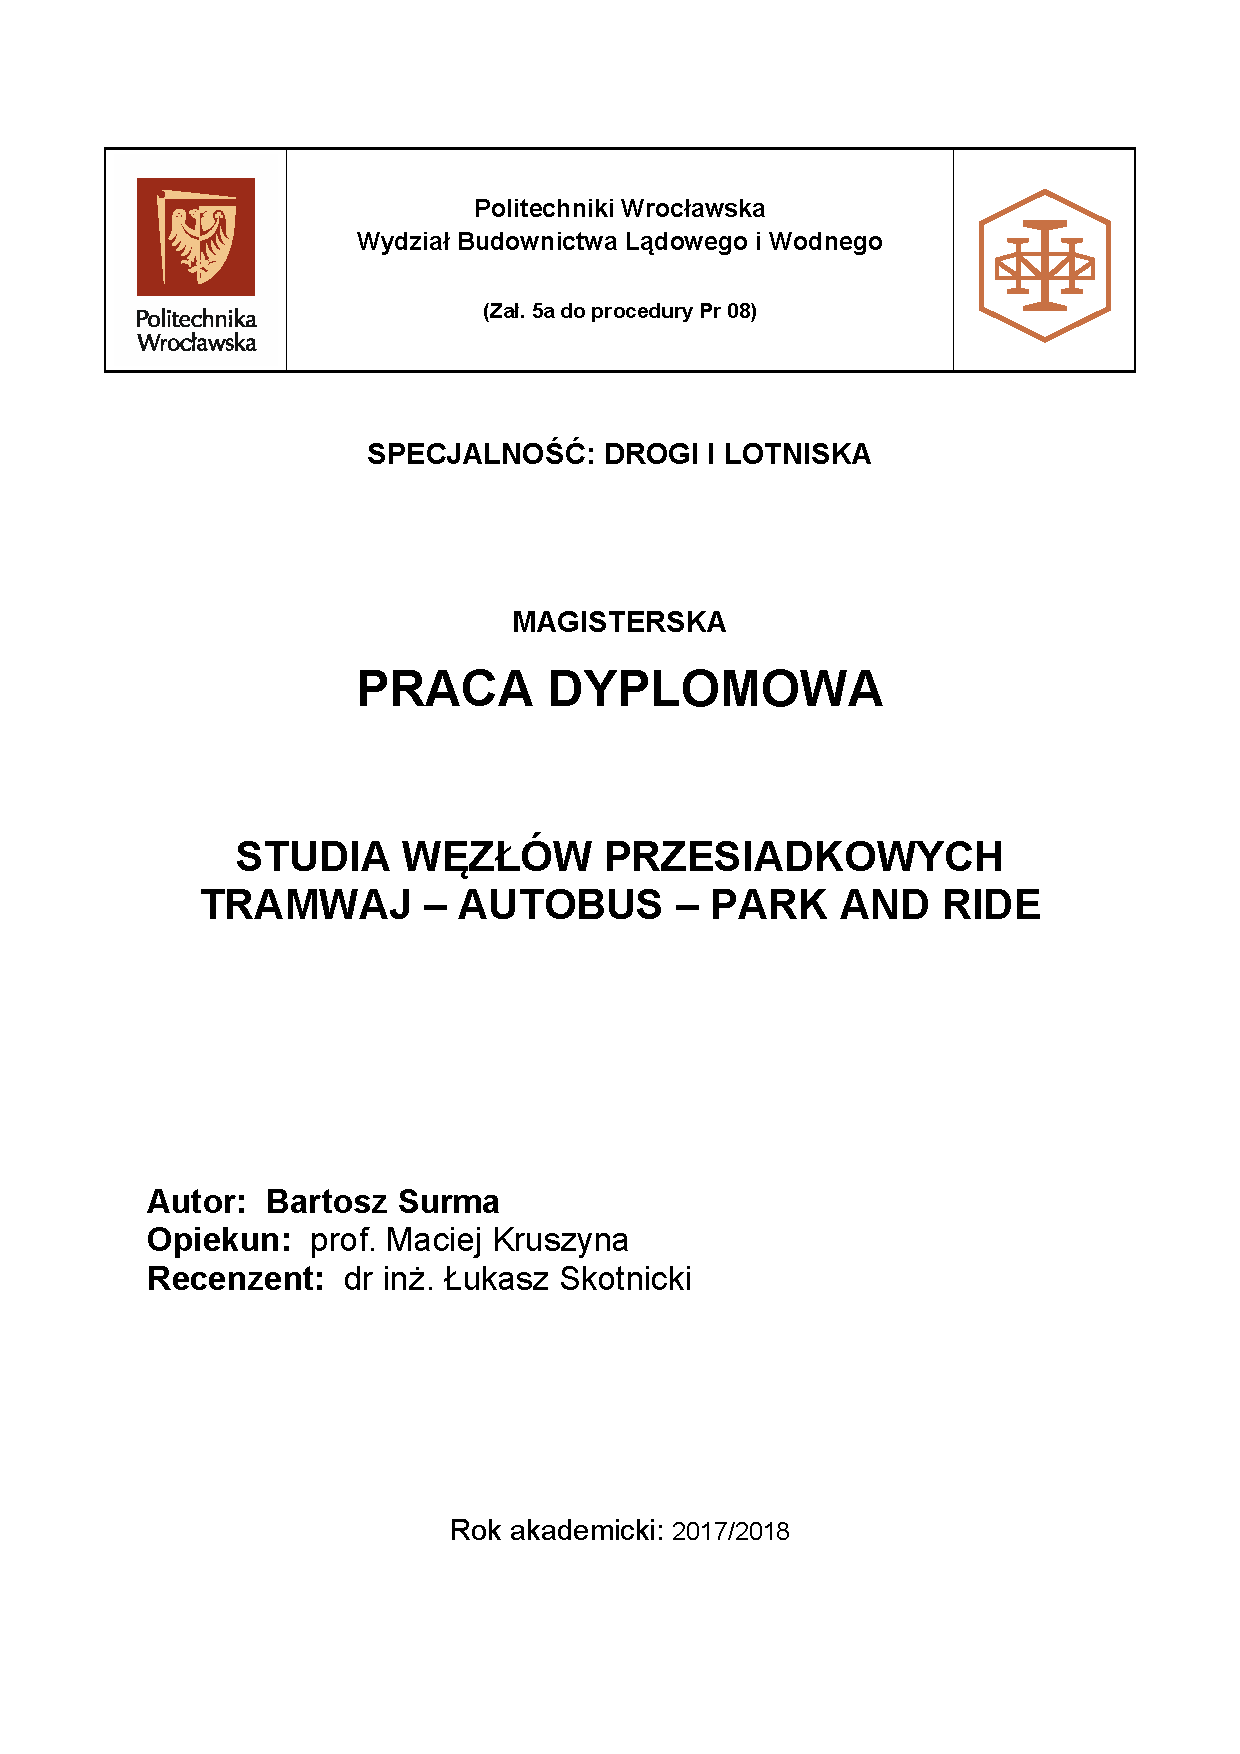
\includepdf{img/strona_tytulowa.pdf}
	\tableofcontents
	\clearpage
	\pagestyle{fancy}

\newcommand{\pnr}{,,Park and Ride''}
\newcommand{\obraz}[4]{	
	\begin{figure}[H]
		\centering
		\caption{#1}
		\includegraphics[width=0.75\textwidth]{#2}\\
		\footnotesize{#3}
		{#4}
	\end{figure}
}

\section{Wprowadzenie}

	\subsection{Cel i zakres pracy}

	\subsection{Idea stosowania węzłów przesiadkowych}
	
	W większości krajów europejskich istnieje prawie całkowita zgoda w kwestii konieczności stosowania transportu publicznego na terenie dużych aglomeracji \cite{guide}. Sprawnie działający zbiorowy transport publiczny jest niezbędny w miastach na terenie starego kontynentu ze względu na typową dla nich zwartą strukturę budynków i centrów miast oraz relatywnie wąskie ciągi drogowe. Osiedla europejskie powstawały w okresie przed rewolucją przemysłową i są nieprzystosowane do obecnego nasilenia ruchu samochodowego, zatem konieczne jest aby część zmotoryzowanego ruchu indywidualnego przejął transport zbiorowy odciążając tym samym sieć drogową miasta. 
	
	Taka postawa jest obecnie najbardziej rozpowszechniona w krajach europejskich, stąd też coraz więcej opracowań na temat rozwoju komunikacji publicznej przygotowywanych zarówno indywidualnie przez państwa europejskie jak i na potrzeby i użytek różnorakich programów rozwojowych proponowanych przez Unię Europejską (przykładowo europejski projekt GUIDE Urban Interchanges oraz tzw. ,,Biała księga transportu EU''). Sprawny i rozbudowany system transportu publicznego działa na korzyść miasta na wiele sposobów: zmniejszając hałas i zanieczyszczenie towarzyszące dużej liczbie pojazdów indywidualnych, zmniejszając zatłoczenie sieci drogowej oraz liczbę wypadków drogowych \cite{szarata} a także zwiększając integrację mieszkańców i atrakcyjność śródmieścia \cite{guide}.  
	
	Wydawać by się mogło, że wiele z tych problemów (w szczególności kongestię ulic i dróg) można rozwiązać rozbudowując sieć drogową miasta, poszerzając ulice, dodając nowe pasy ruchu, zwiększając dopuszczalną prędkość ruchu czy tworząc nowe połączenia między wybranymi osiedlami w mieście. Podejście to było bardzo popularne jeszcze niedawno, szczególnie w Stanach Zjednoczonych, gdzie nawet relatywnie małe aglomeracje mają imponujące połączenie z siecią dróg szybkiego ruchu, a nierzadko istnieje możliwość bezpośredniego wjazdu do centrum z takiej drogi (Dallas TX, Denver CO, Detroit MI). Ogromne węzy drogowe i rozbudowane autostrady to częsty widok w USA przy jednocześnie miernej infrastrukturze transportu zbiorowego. Stan ten w dużej mierze miał swój początek w latach trzydziestych, kiedy to prezydent Roosevelt zapoczątkował serię programów rozbudowy infrastruktury pod nazwą ,,Nowy Ład'' (ang. New Deal), których realizacja znacząco wpłynęła na wskaźnik zmotoryzowania Amerykanów i zepchnęła transport publiczny w cień \cite{makarova}.

	Okazuje się jednak, że takie podejście często ma odwrotny skutek. Przepustowość dodana przez nowe ulice i drogi szybkiego ruchu generuje większy ruch pojazdów. Zjawisko to sformułowane zostało już w 1977 roku przez Davida Lewisa oraz Martina Mogridge'a znane jako \emph{Prawo Lewisa-Mogridge'a}. Jest to teoria mówiąca, że zwiększanie przepustowości dróg nie prowadzi do mniejszego zatłoczenia bowiem liczba samochodów będzie dążyć do wypełnienia nowej dostępnej przestrzeni \cite{prawo-lewisa}. Nie powinno zatem dziwić to, że najbardziej zatłoczone miasta w Stanach Zjednoczonych to często te z największą ilością dróg szybkiego ruchu i naziemnych węzłów drogowych jak na przykład Los Angeles czy Dallas, pomimo ich prostego układu (siatka krzyżujących się arterii) i szerokich ulic.
	
	%\obraz{Przykład węzła drogowego w centrum miasta -- Los Angeles}{Gardena_freeway}{źródło: Asisbiz World Photographs: \url{http://www.asisbiz.com}}
	
	W Europie, gdzie miasta są zdecydowanie starsze niż amerykańskie, takie podejście było niemożliwe, dzięki czemu obecnie widać znacznie większe naciski na działający i sprawny system transportu zbiorowego. Nie oznacza to jednak, że miasta europejskie nie mają problemów z zatłoczeniem. Bardzo dużym problemem jest niezoptymalizowany układ dróg, mający swe początki przed erą motoryzacyjną, wąskie i zabudowane ulice oraz koncentracja usług i najważniejszych ośrodków generujących ruch w ścisłym centrum miasta (przykładowo, pomimo zaledwie 1,7 miliona mieszkańców Warszawa jest na 42. miejscu pod względem zatłoczenia wg pomiarów popularnego na całym świecie systemu nawigacji TomTom \cite{tomtom}). Widać więc wyraźnie potrzebę stosowania i rozwoju usług transportu publicznego, który może być dobrą, a czasem i lepszą, alternatywą dla ciągłego rozwoju sieci drogowej. 
	
	Problemem wielu miast nie jest jednak tylko ruch generowany stricte przez nie. W obecnych czasach, mogąc korzystać z samochodów, ludzie podejmują się pracy z dala od miejsca zamieszkania, a największe możliwości zatrudnienia znajdują się właśnie w miastach, które muszą poradzić sobie z nowym ruchem związanym z podróżami dom-praca-dom mieszkańców podmiejskich osiedli oraz okolicznych wsi. Pojazdy te często bardziej wpływają na zatłoczenie ulic ponieważ korzystają z sieci drogowej miasta dłużej mając do przejechania dłuższą trasę. W związku z tym konieczny jest sprawnie działający system transportu zbiorowego mogący obsłużyć nie tylko pasażerów mieszkających w mieście, ale także i spoza niego. 
		
	Najważniejszą częścią takiego systemu jest węzeł komunikacyjny, czyli miejsce, gdzie łączą się i spotykają co najmniej dwa typy sieci transportowych (na przykład transport samochodowy i autobusowy, transport kolejowy lub tramwajowy czy pasażerski transport morski lub lotniczy). Od płynności działania takiego węzła zależy w dużej mierze jakość działania układu transportowego, jeśli nie całego to na pewno najbliższej jego części \cite{urbanistyka}. 
	
	W świetle polskiego prawa węzeł zintegrowany jest to ,,miejsce umożliwiające dogodną zmianę środka transportu wyposażone w niezbędną dla obsługi podróżnych infrastrukturę, w szczególności: miejsca postojowe, przystanki komunikacyjne, punkty sprzedaży biletów, systemy informacyjne umożliwiające zapoznanie się zwłaszcza z rozkładem jazdy, linią komunikacyjną lub siecią komunikacyjną'' \cite{ustawa_transport}.
	
	\subsection{,,Park and Ride''}
	
	Biorąc pod uwagę konieczność obsłużenia pasażerów spoza aglomeracji, nie dziwi szybkie pojawienie się koncepcji stworzenia węzłów sieci transportu zbiorowego oferujących połączenia komunikacji zbiorowej z przedmieść do centrów dużych miast. Stąd niedaleko do obecnego systemu \pnr{}, którego istotą jest zachęcenie podróżujących do pozostawienia pojazdu na parkingu, usytuowanego blisko stacji, pętli lub przystanku, ale jednocześnie na terenie łatwo dostępnych przedmieść miasta, aby opłacalne było skorzystanie z oferowanych przez komunikację publiczną połączeń w kierunku centrum zamiast kontynuowania podróży samochodem \cite{szarata}.	
	
	Węzły przesiadkowe wyposażone w \pnr{} charakteryzują się rozbudowanym parkingiem mogącym pomieścić od kilkudziesięciu do kilkuset pojazdów w bliskiej odległości od przystanków i dworca. Rolą tych miejsc jest zachęcenie kierowców do pozostawienia pojazdu i skorzystania z komunikacji publicznej. Węzły tego typu najczęściej usytuowane są na przedmieściach, w odległości co najmniej kilku kilometrów od centrum. Zbyt bliskie położenia zmniejsza atrakcyjność przesiadki \cite{szarata}.
	
	Za nieoficjalne początki systemu \pnr{} można uznać parking dla samochodów przy dworcu kolei podmiejskiej w Filadelfii, wybudowany już w 1927 roku, jednakże za pierwszy zaprojektowany i zrealizowany przykład systemu \pnr{} we współczesnej formie należy uznać mieszczący się w Oxfordzie, który otworzony w latach 60., obchodził niedawno swoje 40 urodziny. Początkowo był to parking dedykowany dla podróżujących, którzy mogli przesiąść się na autobusy spółki Oxford Bus Company oferującej połączenia na drodze szybkiego ruchu A34. System ten był dostępny jedynie rok, ale jego idea została użyta ponownie w roku 1973 kiedy to uruchomiono Redbridge Car Park obsługujący ruch autobusowy w kierunku centrum Oxfordu \cite{oxford}.
	
	\obraz{Schemat rozmieszczenia węzłów z systemem \pnr{} w Oxfordzie}%
	{oxford}{źródło: Oxfordshire County Council: \url{https://www.oxfordshire.gov.uk/cms/content/park-and-ride-locations}}
	
		Konieczność zastosowania takiego rozwiązania wynikała z ogromnych problemów z zatłoczeniem miasta w latach 50. i 60. System ten przyjął się i okazał atrakcyjną alternatywą dla kierowców. Na chwilę obecną Oxford posiada pięć głównych parkingów \pnr{} oferujących ponad 5000 miejsc postojowych, zlokalizowanych na obrzeżach miasta i zapewniających połączenie autobusowe do centrum miasta oraz do najważniejszych punktów takich jak chociażby szpitale \cite{oxford2}.
		
	Wzorując się na sukcesie systemu w Oxfordzie, a także niedługo później w Leicester i Nottingham, w Wielkiej Brytanii pojawiało się coraz więcej miejsc oferujących wygodną przesiadkę w komunikację zbiorową. Do lat 90. własne węzły przesiadkowe wyposażone w parking posiadały już takie miasta jak Bath, Chester, Canterbury, Cambridge, Exeter, Norwich, Preston i York \cite{rps}. Przyczyniło się do tego także w dużej mierze wydanie przez angielski departament środowiska dokumentu, w którym \pnr{} był zalecany jako korzystne rozwiązanie dla miast. Popularność systemu w Wlk. Brytanii najlepiej uwidacznia wzrost liczby parkingów w okresie ostatnich 30 lat, co widać na rysunku \ref{pnr_sites}.
	
	\begin{figure}[H]
		\centering
		\caption{Liczba węzłów przesiadkowych z systemem \pnr{} w Wlk. Brytanii}
		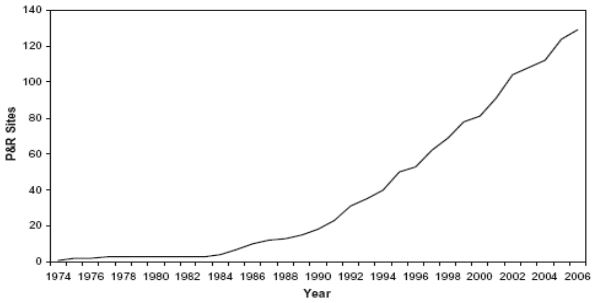
\includegraphics[width=0.75\textwidth]{pnr_sites}\\
		\footnotesize{źródło: Richard Stacey. \emph{The effectiveness and sustainability of Park and Ride}, str. 3. \cite{rps}}
		\label{pnr_sites}
	\end{figure}
	
	Rozwiązanie to szybko przeniosło się do innych krajów kontynentu. W wielu miastach liczba miejsc parkingowych dedykowanych pod \pnr{} jest wyjątkowo wysoka. W 2009 roku niekwestionowanym liderem wśród miast europejskich był Rzym z liczbą miejsc postojowych w ramach \pnr{} przekraczającą 12 800. W ogólnym rankingu bardzo wysoko znajdują się miasta niemieckie: Hamburg -- 9 409 miejsc postojowych, Monachium -- 7 128, Kolonia -- 5 570 i Berlin -- 4 947. Wyprzedzają je jedynie Wiedeń (6 226 miejsc) i Paryż (5 849). Jeśli spojrzeć na liczbę miejsc parkingowych w stosunku do liczby mieszkańców, to wszystkie miasta europejskie mają ten wskaźnik na poziomie od 0 do 6 miejsc postojowych na 1000 mieszkańców z wyjątkiem Luksemburgu (47.7 miejsc na 1000 mieszkańców) oraz Genewy (26.1 miejsc na 1000 mieszkańców) \cite{eurotest}.
	
	O ile wszystkie wymienione miasta tworzyły swoje węzły przesiadkowe w podobnym okresie -- tj. w czasie ostatnich dwudziestu, trzydziestu lat, to jednak są między nimi znaczące różnice w podejściu do problemu jakim jest sprawnie działający węzeł z \pnr{}. Różnice te są widoczne już na stadium projektowania i to na poziomie tego samego kraju -- dla przykładu, w Berlinie oczekiwaną odległością jaką skłonni są przejść piesi w ramach węzła jest około 800 metrów, z kolei w Kolonii to już tylko 100-200 metrów, znacząco mniej. Najmniejsza zgoda w Europie panuje w temacie opłat parkingowych. W Niemczech wszystkie placówki \pnr{} są bezpłatne, przeciwnie w miastach takich jak Genewa, Praga, Sztokholm czy Wiedeń, gdzie wszystkie są odpłatne. W większości miast nie ma jasno określonych cen, różnią się one w zależności od lokalizacji parkingu \cite{eurotest}.
	
	Jak widać na rysunku \ref{pnr_europe} największe zainteresowanie system \pnr{} zyskał w krajach Europy Centralnej i Wielkiej Brytanii (która jest prekursorem tego rozwiązania). Jest to jednak trend, który może ulec zmianie. Coraz więcej miast europejskich zmaga się z problemami zatłoczenia oraz narastającej liczby samochodów i zamierza rozwiązać ten problem właśnie za pomocą \pnr{}. Na atrakcyjność systemów P+R wpływa również pomoc finansowa płynąca z Unii Europejskiej, która wspiera takie rozwiązania. Wiele krajów wschodniej Europy korzystając ze współfinansowania jest w stanie wyposażyć swoje miasta w systemy stosowane w Europie zachodniej. Przykładowo stolica Słowenii, Lublana, ma zostać wyposażona w dodatkowe 23 centra P+R, finansowane wspólnie przez urząd miasta i Europejski Fundusz Spójności. 
	
	\obraz{Ogólny poziom zaadoptowania systemu \pnr{} w wybranych miastach europejskich (stan na rok 2011), gdzie 1 oznacza bardzo niski, a 5 bardzo wysoki}{pnr_europe}{źródło: Marc Dijk, Carlos Montalvo: \emph{Policy frames of Park-and-Ride in Europe}. \\,,Journal of Transport Geography''. nr 19/2011. \cite{dijk}}{\label{pnr_europe}}
	
	Pierwsze próby wprowadzenia parkingów \pnr{} w Polsce miały miejsce w latach dziewięćdziesiątych w Krakowie. Były to próby nieudane, ze względu na złą lokalizację systemu zbyt blisko centrum przez co parkingi te służyły jedynie jako miejsce postojowe a nie węzeł przesiadkowy. W związku z tym ulegały one stopniowej likwidacji aż do roku 2003. Kiedy w Krakowie system likwidowano, w Warszawie w 2006 roku rozpoczęto budowę systemu odpowiednio zlokalizowanych parkingów strategicznych. Cały system był planowany już od 1995 roku, a oddany został do użytku w roku 2007. W jego skład wchodzi obecnie 14 parkingów mogących pomieścić ponad 4200 samochodów osobowych \cite{rybczynska}. Z kolei we Wrocławiu na chwilę obecną funkcjonuje siedem parkingów \pnr{} oraz są plany budowy dodatkowych jedenastu. Prawie wszystkie z nich znajdują się na południu miasta (dzielnice Krzyki i Grabiszyn) oraz na północnym zachodzie (osiedla Kosmonautów i okolice stadionu miejskiego).
	
	\subsection{Charakterystyka węzłów przesiadkowych}
	
	Za węzeł przesiadkowy możemy przyjąć miejsce, gdzie istnieje możliwość przesiadki pomiędzy co najmniej dwoma środkami podróży. Z racji, że rodzajów komunikacji indywidualnej jak i zbiorowej jest wiele, tak samo można uznać, że wiele jest rodzajów węzłów przesiadkowych. Analiza istniejących węzłów w Szwajcarii daje podstawę do uznania pięciu ich głównych typów \cite{standardy_szwajcarskie}:
	\begin{itemize}
		\item Duże dworce kolejowe o znaczeniu międzynarodowym. Są to obiekty skupiające wiele różnych form transportu o dużej częstotliwości, zapewniające obsługę bardzo dużej liczby pasażerów. W obiektach tego typu znajduje się duża liczba dostępnych usług oraz są one łatwo dostępne dla praktycznie każdego.
		\item Regionalne dworce kolejowe, które skupiają się głównie na międzymiastowym ruchu krajowym. Obsługują one mniejszą liczbę pasażerów, choć posiadają bardzo wiele połączeń regionalnych, przede wszystkim autobusów zapewniających transport z okolicznych miejscowości.
		\item Lokalne dworce kolejowe obsługujące połączenia regionalne w obrębie danego regionu. Ważna dla takich obiektów jest ich dostępność dla ruchu pieszego i rowerowego oraz możliwość dłuższego postoju samochodów. Takie dworce mają również bardzo duże znaczenie dla połączeń autobusowych dla danego miasta i służą jako punkt przesiadkowy dla podróżujących do pracy. 
		\item Czwartym typem węzłów są punkty przesiadkowe obsługujące ruch lokalny w obrębie danego miasta z wyłączeniem ruchu kolejowego. Są to głównie węzły tramwajowe i autobusowe z dużą liczbą przystanków z których linie kursują z dużą częstotliwością. Takie węzły charakteryzuje duży ruch pieszych. 
		\item Ostatnim typem węzłów są punkty typu \pnr{}, które obsługują jedną lub kilka linii autobusowych bądź tramwajowych zapewniających dojazd do centrum i służą głównie podróżom do pracy. Charakteryzują się dużą liczbą miejsc postojowych dla samochodów i rowerów.
	\end{itemize}
	
		Jest to ogólny podział węzłów przesiadkowych, przyjęty w Szwajcarii ale doskonale sprawdzający się na terenie całej Europy, w tym także w Polsce. Fakt wyszczególnienia węzłów typu \pnr{} jako osobnej grupy węzłów przesiadkowych wynika z różnic jakie posiadają obiekty takiego typu w stosunku do innych rodzajów węzłów, tj. przyjmowanie podróżujących ze ściślej określonych obszarów w okolicach P+R i obsługa połączeń głównie w jednym kierunku, do centrum miasta. Pomimo tak precyzyjnych warunków funkcjonowania parkingi \pnr{} mogą się od siebie znacząco różnić. Dopuszcza się istnienie zarówno małych ośrodków obsługujących czasem tylko jedną linię tramwajową bądź autobusową i posiadających kilkanaście miejsc parkingowych, jak i istnienie bardzo dużych kompleksów z przystankami dla wielu linii autobusowych i tramwajowych oraz z parkingami oferującymi kilkaset miejsc postojowych i wiele dodatkowych usług takich jak zatoki ,,Kiss and Ride'', stanowiska dla rowerów indywidualnych (,,Bike and Ride'') jak i rowerów miejskich (np. system Veturilo). 

\section{Projektowanie węzłów przesiadkowych}

	\subsection{Czynniki wpływające na atrakcyjność węzłów przesiadkowych}

	Węzeł przesiadkowy to miejsce, gdzie co najmniej dwa środki transportu (zbiorowego lub indywidualnego) łączą się, umożliwiające wygodną przesiadkę. Jest to kluczowy punkt funkcjonowania sieci transportowej miasta. Od efektywności obsługi pasażerów na węzłach zależy w dużej mierze efektywność całej sieci \cite{urbanistyka}. W związku z tym konieczne jest usystematyzowanie i określenie wymagań i tzw. dobrych praktyk dotyczących projektowania takich węzłów, jak i ich lokalizowania. 
	
	Najważniejszym czynnikiem efektywności węzła jest jego lokalizacja. Planując nową inwestycję należy wziąć pod uwagę wiele czynników, takich jak główne kierunki ruchu w sieci drogowej miasta i jej miejscowe zatłoczenie, schemat komunikacji zbiorowej i dostępną liczbę połączeń, spodziewaną liczbę użytkowników węzła, przestrzeń dostępną do zagospodarowania i ewentualną rozbudowę oraz wpływ wybranej lokalizacji na okolicę i środowisko \cite{icaen}. Jeśli zaś chodzi o sam proces projektowania, kluczowym jest wzięcie pod uwagę kilku czynników, które wpływają na atrakcyjność i wygodę korzystania z danego węzła. Czynniki te to \cite{icaen} \cite{metodyka} \cite{poznan} \cite{kazimierczyk}:
	\begin{itemize}
		\item Dostępność miejsc parkingowych, zarówno dla kierowców jak i rowerzystów, dobrana tak aby poszukiwanie miejsca postojowego nie zabierała za dużo czasu. Miejsca rowerowe powinny być dobrze oznaczone, łatwo dostępne i w dostatecznej liczbie, aby zachęcić rowerzystów do pozostawienia roweru i skorzystania z komunikacji zbiorowej. 
		\item Dobrze zoptymalizowany obszar ruchu pojazdów, który minimalizuje liczbę wypadków i czas poszukiwania miejsca parkingowego. Zaprojektowany tak, aby uniknąć powstawania kolizji i niebezpiecznych zdarzeń, ale jednocześnie aby był intuicyjny i nieskomplikowany w odczycie przez kierowców zapewniając łatwość wjazdu i wyjazdu na parking oraz poszukiwania miejsca i pojazdu.
		\item Odpowiednia dostępność terenu przeznaczonego na infrastrukturę węzła przesiadkowego wraz z parkingiem, aby potoki piesze, autobusowe i samochodowe nie mieszały się, co może prowadzić do opóźnień ruchu oraz do niebezpiecznych sytuacji z udziałem pieszych i pojazdów.
		\item Sprawność węzła, czyli odpowiednia liczba stanowisk postojowych i dobra organizacja ruchu pojazdów gwarantująca wysoką przepustowość.
		\item Odpowiednie oznakowanie całego kompleksu, w taki sposób aby było ono intuicyjne dla pieszych i kierowców. Oznacza to odpowiednie oznakowanie stref parkingowych -- wjazdów, wyjazdów i miejsc postojowych, stref przystankowych, stref ruchu autobusów, tramwajów i kolei, odpowiednie oznakowanie ciągów pieszych, obecność tablic wskazujących kierunek do miejsc przystankowych oraz tablic informujących o dostępnych połączeniach i czasach odjazdów.
		\item Dobrze zorganizowany układ chodników, przejść przez jezdnie i innych ciągów pieszo-rowerowych, dający poczucie bezpieczeństwa i komfortu dla korzystających. Odpowiednio zoptymalizowany układ przejść i chodników zwiększa czytelność węzła dla pieszych.
		\item Obecność urządzeń służących poprawie bezpieczeństwa: oświetlenie, bariery odgradzających miejsca niebezpieczne i ulice, poręcze przy schodach i rampach, systemu obserwacji za pomocą kamer, ewentualny punkt ochrony, ale także i odpowiednie nawierzchnie chodników (zapobiegające poślizgom) oraz systemy odprowadzania wody. 
		\item Dbałość o wysoką estetykę kompleksu -- tj. duża liczba zieleni niskiej i wysokiej, fragmentów zacienionych, obecność ławek, koszów na śmieci, oświetlenia, miejsc zadaszonych czy wiat służących oczekiwaniu na komunikację miejską. Konieczne jest dbanie o czystość dróg i chodników i ciągła kontrola stanu infrastruktury węzła.
		\item Zagwarantowanie miejsc pod działalność usługową taką jak kioski, szalety miejskie oraz małe sklepy. Zalecenia szwajcarskie mówią nawet o dostępności przechowalni bagażu oraz kawiarniach \cite{standardy_szwajcarskie}.
	\end{itemize}	 
	
	Spełnienie powyższych założeń znacząco zwiększa atrakcyjność zaprojektowanego węzła przesiadkowego tym samym zwiększając liczbę jego użytkowników. Idealną sytuacją byłoby spełnienie wszystkich, jednak często sytuacja projektowa na to nie pozwala ze względu na skomplikowane warunki terenowe lub sytuację finansową. W związku z tym konieczne jest wytypowanie tych czynników, które mają największe znaczenie dla korzystających z węzła pasażerów. 
	
	Badania przeprowadzone na grupie 158 osób korzystających z parkingów Park \& Ride w Sztokholmie (parkingi Vällingby, Åkeshov oraz Råcksta) polegały właśnie na ocenie czynników, które mogłyby wpływać na atrakcyjność parkingów P+R. Okazało się, że najważniejszym czynnikiem dla większości ankietowanych była szeroko pojęta kwestia bezpieczeństwa, zarówno własna, jak i samochodu. I pierwsza i druga  uzyskały średnio wagę 4,7 w skali od 1 do 5. Częstotliwość kursowania komunikacji zbiorowej oraz dostępność miejsc parkingowych były niewiele dalej uzyskawszy ocenę 4,6 w tej samej skali. Pozostałe czynniki, takie jak intuicyjność węzła (czy wszystkie formy transportu odjeżdżają z tego samego przystanku) oraz obecność wszelkiego rodzaju usług (takich jak sklepy i kioski) miały zdecydowanie mniejszy wpływ na atrakcyjność węzła/parkingu. W skali pięciopunktowej osiągały odpowiednio 3,6 oraz 2,0 punktu \cite{olsson}.
		
	Przy ocenie czynników negatywnych największy wpływ ma odległość pomiędzy miejscem parkingowym a przystankiem (4,4 punktu na 5 możliwych) i jest on decydującym. Pozostałe czynniki takie jak trudność w znalezieniu parkingu P+R (3,5 pkt.) oraz dostępność miejsc parkingowych (3,4 pkt.) miały zauważalnie mniejszy wpływ na wybór komunikacji zbiorowej. Co ciekawe w tym samym badaniu 78\% ankietowanych powiedziało, że gdyby nie znalazło miejsca parkingowego najprawdopodobniej pojechałoby do innego parkingu w bliskiej okolicy a jedynie 15\% zdecydowałoby się na podróż samochodem do celu \cite{olsson}.
		
	Po analizie wyników można zauważyć, że najważniejszymi czynnikami przy projektowaniu są bezpieczeństwo oraz odległość pomiędzy miejscami parkingowymi i przystankiem. Zgadza się to również z podobnymi badaniami przeprowadzonymi w innych krajach Unii Europejskiej. W ankietyzacji mieszkańców Goteborgu (580 tys. rezydentów, a zatem liczba bardzo zbliżona do miasta Wrocławia) jednym z najważniejszych czynników była odległość do pokonania pieszo mniejsza niż 300 metrów \cite{gothenburg}. Również zalecenia amerykańskie przy projektowaniu węzłów przesiadkowych zwracają uwagę na konieczność minimalizowania odległości pomiędzy parkingami i przystankami. Zalecane jest lokalizowanie przystanków w centrum całego kompleksu, a jako maksymalną drogę jaką skłonni są pokonać piesi podano odległość 1000 stóp czyli około 305 metrów \cite{florida}. W Polsce również dąży się do minimalizowania tych odległości. W dokumencie przygotowanym dla miasta Poznania dotyczącym koncepcji budowy węzłów przesiadkowych Poznańskiej Kolei Metropolitarnej jako najważniejsze czynniki podaje się te związane z infrastrukturą na terenie węzła czyli: minimalizację odległości do pokonania przez pieszych, minimalizację różnicy poziomów, zalecenie stosowania szerokich i dobrze oświetlonych ścieżek i chodników. Zaleca się także wprost wyznaczenie peronów przystankowych możliwie najbliżej miejsc postojowych a jako praktykę pożądaną podaje się stosowanie peronów umożliwiających przesiadkę ,,drzwi w drzwi'' czyli o maksymalnej odległości koniecznej do przebycia wynoszącej zaledwie parę metrów \cite{poznan}.
	
	Dodatkową informacją na temat czynników charakteryzujących dobrze zaprojektowany węzeł może być także system oceny węzłów przesiadkowych opracowany przez dr Piotra Olszewskiego, dzielący kryteria na dwie grupy: wskaźniki ciężkie (integracja przestrzenna, dostępność dla osób niepełnosprawnych i wewnętrzna logika węzła czyli czytelność) oraz wskaźniki lekkie (informacja pasażerska, bezpieczeństwo osobiste, bezpieczeństwo wynikające z ruchem pojazdów -- kolizje oraz obecność dodatkowych funkcji) \cite{raport-vip}. Również i z tych wskaźników wynika, że zadowalająca pieszych odległość do przejścia na terenie węzła to główne kryterium przy ocenie jakości węzła przesiadkowego. 
	
	Biorąc pod uwagę powyższe informacje wydaje się oczywistym, że ruch pieszych na terenie węzła przesiadkowego ma charakter priorytetowy. W związku z tym konieczne jest ustalenie odpowiedniej hierarchii dla poszczególnych użytkowników węzła. Jednym z proponowanych może być ten przedstawiony na rysunku \ref{access-hierarchy}.
	
	\begin{figure}[H]
		\centering
		\caption{Hierarchia użytkowników węzłów przesiadkowych}
		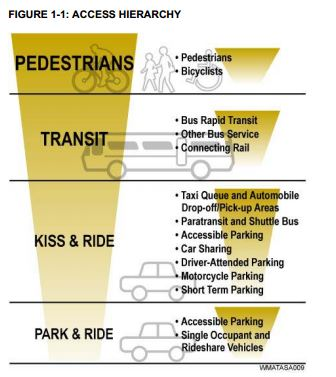
\includegraphics[width=0.5\linewidth]{access_hierarchy}\\
		\footnotesize{źródło: Washington Metropolitan Area Transit Authority, \emph{Guidelines for station site and access planning}, Sierpień 2005 \cite{guidelines_washington}}
		\label{access-hierarchy}
	\end{figure}
	
	Najważniejszy priorytet, jak już powiedziano, należy się pieszym oraz rowerzystom. Nieprzerwane ulicą oraz intuicyjne i czytelne ciągi pieszo-rowerowe zwiększają bezpieczeństwo na terenie węzła i zachęcają do korzystania z niego. Drugą grupą w hierarchii jest zbiorowa komunikacja publiczna czyli autobusy i tramwaje, które z racji większego zagęszczenia użytkowników na pojazd mają priorytet nad pojazdami indywidualnymi oraz komunikacją publiczną indywidualną, które stanowią grupy trzecią i czwartą. Pojazdy indywidualne, które obecne na terenie węzła są jedynie na krótko (taksówki lub samochody parkujące w ramach systemu ,,Kiss and Ride'') lub zajmują mało miejsca (motocykle lub rowery) stanowią trzecią grupę, stojąc w hierarchii wyżej od samochodów parkujących w ramach systemu \pnr{} \cite{guidelines_washington}.
	
	\subsection{Wskaźnikowa ocena węzłów przesiadkowych}
	
	Ocena jakości węzła przesiadkowego polega głównie na opisowym określeniu jakości poszczególnych kryteriów takich jak układ czy czytelność węzła. Jest to metoda jakościowa nie pozwalająca na bezpośrednie porównanie kilku wariantów danego węzła czy na porównanie różnych rozwiązań zastosowanych w danym mieście. Aby to umożliwić w 2012 roku opracowana została metodyka oceny węzłów na podstawie wskaźników ilościowych pod nazwą Ocena Wskaźnikowa Węzłów Przesiadkowych Transportu Publicznego AMPTI (Assesment Method of Public Transport Interchanges). Jej autorami byli Piotr Olszewski oraz Halina i Piotr Krukowscy. Zaproponowali oni 14 wskaźników podzielonych na dwie grupy: wskaźniki ogólne dotyczące całego węzła oraz wskaźniki szczegółowe dla poszczególnych elementów. Poszczególne wskaźniki pokazano w tabeli \ref{metodyka} \cite{metodyka}. 
	
	Wskaźniki te w większości odpowiadają procentowi elementów, które spełniają przyjęte założenia. Jeśli połowa peronów spełnia kryteria dostępności dla osób starszych i niepełnosprawnych to wartość wskaźnika W.5p wynosi 50\%. W celu określenia wartości poszczególnych wskaźników należy podzielić węzeł na części składowe -- perony oraz dojścia do nich. Przejścia między peronami składają się z trzech elementów: chodnika, przejścia przez jezdnię oraz schodów. Dzieląc wszystkie trasy na elementy składowe możemy obliczyć wartości poszczególnych wskaźników.
	
	\def\malaczcionka#1{\footnotesize{#1}}
	% Table generated by Excel2LaTeX from sheet 'MEtodyka AMPTI'p{0.2\linewidth}p{0.2\linewidth}p{0.5\linewidth}
\begin{table}[H]
  \centering
  \caption{Opis wskaźników w metodyce AMPTI}
			\begin{tabular}{p{0.2\linewidth}p{0.1\linewidth}p{0.625\linewidth}}
			\toprule
			\textbf{Nazwa wskaźnika} & \textbf{Symbol} & \textbf{Opis} \bigstrut[b]\\
			\midrule
			\multicolumn{3}{c}{\textbf{Wskaźniki ogólne dla węzła jako całości}}  \bigstrut\\
			\midrule
			\multirow{3}{\linewidth}{Zwartość węzła} & W.1.1c     & \malaczcionka{Średni ważony czas przejścia pieszego pomiędzy wszystkimi peronami} \bigstrut[t]\\
			           & W.1.1d     & \malaczcionka{Średnia ważona długość przejścia pieszego pomiędzy wszystkimi peronami} \\
			           & W.1.2d     & \malaczcionka{Średnia arytmetyczna długość przejścia pieszego pomiędzy wszystkimi peronami} \bigstrut[b]\\
			\midrule
			Czytelność węzła & W.2        & \malaczcionka{Średni odsetek przystanków i wejść do stacji widocznych z innych przystanków} \bigstrut\\
			\midrule
			Wyposażenie dodatkowe & W.3        & \malaczcionka{Odsetek wszystkich możliwych urządzeń dodatkowych, które są w danym węźle} \bigstrut\\
			\midrule
			\multicolumn{3}{c}{\textbf{Wskaźniki szczegółowe dla elementów węzła}} \bigstrut\\
			\midrule
			\multirow{2}{\linewidth}{Infrastruktura podstawowa} & W.4p       & \malaczcionka{Odsetek peronów, które spełniają kryteria jakości infrastruktury} \bigstrut[t]\\
			           & W.4s       & \malaczcionka{Odsetek segmentów przejść, które spełniają kryteria jakości infrastruktury} \bigstrut[b]\\
			\midrule
			\multirow{2}{\linewidth}{Dostępność dla niepełnosprawnych} & W.5p       & \malaczcionka{Odsetek peronów, które spełniają kryteria dostępności dla starszych i niepełnosprawnych} \bigstrut[t]\\
			           & W.5s       & \malaczcionka{Odsetek segmentów przejść, które spełniają kryteria dostępności} \bigstrut[b]\\
			\midrule
			\multirow{2}{\linewidth}{Bezpieczeństwo osobiste} & W.6p       & \malaczcionka{Odsetek peronów, które spełniają kryteria bezpieczeństwa osobistego} \bigstrut[t]\\
			           & W.6s       & \malaczcionka{Odsetek segmentów przejść, które spełniają kryteria bezpieczeństwa osobistego} \bigstrut[b]\\
			\midrule
			\multirow{2}{1\linewidth}{Bezpieczeństwo w ruchu} & W.7        & \malaczcionka{Średni poziom bezpieczeństwa dla wszystkich przejść przez jezdnie w węźle} \bigstrut\\
			\midrule
			\multirow{2}{1\linewidth}{Informacja pasażerska} & W.8p       & \malaczcionka{Odsetek peronów z dostępną informacją pasażerską} \bigstrut[t]\\
			           & W.8s       & \malaczcionka{Odsetek segmentów przejść z dostępną informacją pasażerską} \\
			\bottomrule
			\end{tabular}%
  \label{metodyka}
  \footnotesize{źródło: Olszewski P., Krukowska H., Krukowski P.,	\emph{Metodyka oceny wskaźnikowej węzłów przesiadkowych transportu publicznego}, ,,Transport miejski i regionalny'' Czerwiec 2014 \cite{metodyka}}
\end{table}%

Wskaźniki zwartości węzła oblicza się na podstawie macierzy poszczególnych wartości (odległości i czasu) dla poszczególnych peronów. Pierwszy ze wskaźników, zwartość węzła, można obliczyć na trzy podane sposoby. Pierwszym z nich jest obliczenie średniej ważonej odległości przejścia pieszego pomiędzy wszystkimi peronami (W.1.1d), obliczanej wg wzoru \ref{eq:ampti1} \cite{metodyka}:
\begin{equation}
\overline{d}=\sum_{i=1}^{n}\sum_{j=1}^{n}p_{ij}d_{ij} \label{eq:ampti1}
\end{equation}

Gdzie $d_{ij}$ -- czas przejścia między peronami $i$ oraz $j$, $p_{ij}$ -- udział przesiadek między peronami $i$ i $j$ czyli stosunek liczby pasażerów przesiadających się pomiędzy danymi peronami do całkowitej liczby użytkowników węzła, $n$ -- liczba czynnych peronów. W przypadku przesiadek na tym samym peronie za odległość, którą musi pokonać pasażer, przyjmuje się równą $1/3$ długości peronu. W przypadku obliczania średniego ważonego czasu przejścia między wszystkimi peronami (W.1.1c) używa się wzoru podobnego do (\ref{eq:ampti1}) z tym, że zamiast drogi $d_{ij}$ przyjmuje się czas $t_{ij}$ przejścia między poszczególnymi peronami. Najmniej dokładnym sposobem określenia zwartości węzła jest arytmetyczna średnia długość przejść między peronami (W1.2d), którą oblicza się wg wzoru \ref{eq:ampti2} \cite{metodyka}:
\begin{equation}
\overline{d3}=\frac{2}{n(n+1)-2K}\sum_{i=1}^{n}\sum_{j=1}^{n}d_{ij} \label{eq:ampti2}
\end{equation}
Gdzie $K$ -- liczba peronów, na których nie mają miejsca przesiadki na tym samym peronie (na przykład perony dla wysiadających), w takim przypadku można przyjąć $d_{ij}=0$.

Czytelność węzła (W.2) określona jest jako średnia liczba przystanków widoczna z każdego przystanku podzielona przez liczbę przystanków pomniejszoną o jeden. Pozwala to określić średni stopień widoczności innych przystanków na obszarze węzła a przez to określić orientację węzła przez użytkowników. W przypadku węzłów wielopoziomowych należy brać pod uwagę odpowiednie oznaczenia wejść lub tuneli prowadzące do danych przystanków. Wyposażenie dodatkowe (W.3) to: zadaszenie peronów i przejść pieszych, ławki, kosze na śmieci, biletomaty, sklepy, toalety, postoje taksówek, stojaki dla rowerów, parkingi \cite{metodyka}. Wartość wskaźnika to procentowa obecność wymienionych urządzeń.

Jakość infrastruktury podstawowej (W.4) to odsetek peronów i przejść spełniających kryteria jakości uznawane w danym mieście, wśród których można wymienić takie jak szerokość peronu lub chodnika, długość peronu przystanku tramwajowego lub autobusowego, jakość
nawierzchni, brak przeszkód w obrębie przystanku, maksymalna wysokość krawężnika czy obecność wiaty. Jeśli nie jest spełniony którekolwiek z podstawowych kryteriów, cały element jest traktowany jako nie spełniający wymogów jakości. Dostępność dla osób starszych i niepełnosprawnych (W.5) to odsetek elementów węzła spełniających założenia dostępności dla pieszych, czyli posiadania: pochylni lub wind w miejscach występowania schodów, poręczy wzdłuż pochylni, ostrzegawczych płytek chodnikowych z wypustkami i kontrastowych oznaczeń wzdłuż krawędzi peronów oraz przed schodami, obniżonych krawężników i płytek ostrzegawczych przy przejściach przez jezdnie oraz sygnałów dźwiękowych na przejściach z sygnalizacją świetlną \cite{metodyka}.  

Wskaźnik bezpieczeństwa osobistego (W.6) określa się jako odsetek elementów węzła posiadających dostateczne oświetlenie i monitoring. Wskaźnik bezpieczeństwa w ruchu (W.7) to średnia z poziomu bezpieczeństwa wszystkich przejść dla pieszych na terenie węzła, przy czym autorzy przyjęli, że różne rodzaje przejść zapewniają odmienne poziomy bezpieczeństwa. Przejścia całkowicie odseparowane od pojazdów, takie jak kładki czy tunele zapewniają 100\% bezpieczeństwa, przejścia z sygnalizacją świetlną bez konfliktów z pojazdami to 70\%, z konfliktami 50\%, przejścia bez sygnalizacji 30\%, zaś przejścia nieoznakowane 0\% \cite{metodyka}.

Ostatnim wskaźnikiem jest jakość informacji pasażerskiej (W.8). Wskaźnik ten oblicza się jako procent elementów węzła zawierających wymagane rodzaje informacji dla pasażerów takie jak: rozkłady jazdy i informacje taryfowe na każdym przystanku, plan węzła i jego otoczenia, schemat sieci danego miasta, oznakowanie kierunkowe na peronach i rozgałęzieniach przejść pieszych \cite{metodyka}.

W 2015 roku autorzy metodyki uzupełnili ją dodatkowym wskaźnikiem -- stopniem swobody ruchu pieszych na obszarze węzła. Określa się go jako stosunek odcinków zatłoczonych do wszystkich dostępnych na danym węźle. Zatłoczony ciąg pieszy to taki o poziomie swobody ruchu na poziomie D lub gorszym. O poziomach swobody ruchu szerzej napisane jest w rozdziale \ref{sec:ciagi_piesze}. Kryterium swobody ruchu na terenie peronów przyjmuje się jako minimum 0,93 m2/osobę przy odjęciu dwóch pasów po 0,5 metra od krawędzi peronów \cite{metodyka2}.  

Badanie jakości węzła przesiadkowego przeprowadza się w formie audytu wykonywanego na działającym już węźle i pozwala ilościowo określić jakość poszczególnych kryteriów ważnych dla pasażerów. Nie jest możliwe określenie poszczególnych wskaźników na projektowanym węźle ale ich znajomość pozwala na wzięcie ich pod uwagę podczas projektowania.

	\clearpage
	\subsection{Wybór lokalizacji z punktu widzenia użytkowników ,,Park and Ride''}
	
	Z racji, że większość projektowanych obecnie węzłów przesiadkowych wyposażonych jest w system \pnr{} konieczne jest rozważenie problemu jakim jest lokalizacja parkingu. Podchodząc od strony użytkowników systemu \pnr{} lokalizacja całego węzła ma bardzo duże znaczenie i często to kierowcy poruszający się po danej aglomeracji sami są w stanie wskazać miejsca, które ich zdaniem nadawałyby się najlepiej na węzeł z systemem \pnr{}. Aby wskazać miejsca najbardziej atrakcyjne dla kierowców można także zidentyfikować te, gdzie tworzą się naturalne punkty P+R \cite{guide}, tj. gdzie kierowcy zostawiają swoje pojazdy na parkingach należących do okolicznych sklepów i innych usług, a następnie przesiadają się w komunikację publiczną. Przykładem takiego miejsca we Wrocławiu są okolice Centrum Marino na północy, z którego parkingu korzysta wielu kierowców z okolicznych gmin wrocławskich i trzebnickich zostawiając tam pojazd i przesiadając się na linie 1, 7 lub 15 jadące w stronę centrum miasta. 
	
	Kolejnym, naturalnym wręcz, kryterium przy wyborze lokalizacji P+R jest pętla lub miejsce połączenia kilku linii autobusowych bądź tramwajowych, z których korzysta duża liczba okolicznych mieszkańców. Takie punkty automatycznie są w stanie zapewnić połączenie w wielu różnych kierunkach znacząco zwiększając atrakcyjność węzła oraz liczbę korzystających z niego osób. Podobnym podejściem jest także bazowanie na obecności dużych węzłów i skrzyżowań drogowych łączących główne trasy w mieście. Są to ulice najwyższych kategorii, często kilkupasowe, stanowiące bezpośrednie trasy z i do centrum. Czynniki te gwarantują dużą liczbę użytkowników projektowanego węzła \pnr{}. Taki sam wpływ mają również znacznej wielkości skupiska ludzi, czyli duże osiedla na obrzeżach miast, które są generatorami znacznego ruchu samochodowego typu praca-dom. Przy wyborze odpowiedniego miejsca wskazane jest także skupienie się na istniejących lub przyszłych planach rozbudowy sieci drogowej miasta oraz komunikacji publicznej \cite{guide}. 
	
	Po rozważeniu podanych wyżej czynników może się okazać, że istnieje wiele miejsc, które nadają się na potencjalną lokalizację inwestycji z punktu widzenia użytkowników \pnr{}. W związku z tym konieczna jest analiza i ocena poszczególnych wariantów. Należy tutaj wziąć pod uwagę \cite{guide} \cite{metodyka}:
	\begin{itemize}\setlength\itemsep{0em}
		\item Przede wszystkim, dostępność komunikacji publicznej. Jest to najważniejszy czynnik wpływający na wybór lokalizacji. 
		\item Teoretyczną dostępność projektowanego obiektu z poziomu okolicznych ulic oraz jego wpływ na ruch samochodowy. Ważne jest aby nowy obiekt nie wpływał negatywnie na swobodę ruchu na okolicznych ulicach i nie generował dodatkowego zatłoczenia.
		\item Okolicę wybranej lokalizacji, dostępność terenu pod zabudowę i wymaganą liczbę miejsc postojowych. W niektórych przypadkach można rozważyć rozbicie całego kompleksu na kilka mniejszych podjednostek, pod warunkiem ciągłego zapewnienia komfortu użytkowania.
		\item Dostępność okolicy dla pieszych i rowerzystów. Jest to grupa użytkowników, która jest skłonna pokonać najkrótszą odległość aby skorzystać z proponowanego węzła przesiadkowego. 
		\item Dostępność obiektu dla kierowców, intuicyjność wybranej lokalizacji. Źle dobrana (na przykład w zbyt dużej odległości od najważniejszych szlaków samochodowych w mieście) będzie negatywnie wpływać na atrakcyjność węzła.
		\item Obecne zatłoczenie dróg dojazdowych do centrum miasta. Lokalizacja węzła przy bardzo zatłoczonych ulicach jest w stanie zdemotywować kierowców do korzystania z niego ze względu na brak zauważalnego zysku czasu przy skorzystaniu z komunikacji publicznej. 
		\item Możliwość dalszego rozwoju już zbudowanego węzła przesiadkowego biorąc pod uwagę przyszły rozwój okolicy (rozbudowa osiedli mieszkalnych) oraz komunikacji zbiorowej (dodatkowe linie i nowe typy połączeń).
		\item Ostatecznie, zaleca się także zbadanie opinii publicznej aby ustalić priorytety przy wyborze miejsca inwestycji.		
	\end{itemize}
	
%	W celu ilościowej analizy potencjalnych lokalizacji można również skorzystać z metody punktowej zaproponowanej przez American Association of State Highway and Transportation Officials (AASHTO) w pracy pt. ,,Design Guide for High Occupancy Vehicle (HOV) and Public Transfer Facilities.'' \cite{guide} gdzie podane czynniki ocenia się w skali od 0 do 10 punktów. W tabelach \ref{aashto_tab1} oraz \ref{aashto_tab2} podano kryteria przy ocenie wybranych czynników.
%	
%	Niektóre z podanych czynników mogą być trudne do oznaczenia. Przykładowo, bez znajomości dokładnych pomiarów ruchu uwzględniających punkt początkowy i końcowy każdego pojazdu bardzo trudno jest określić odległość miejsca zamieszkania kierowców od potencjalnej lokalizacji P+R, a ma to duże znaczenie. Szacuje się, że 50\% użytkowników danego węzła ma odległość do miejsca zamieszkania mniejszą niż 5 mil, a 90\% mniejszą niż 10 mil. Oznacza to, atrakcyjność obiektu znacząco spada wraz ze wzrostem odległości \cite{guide}.
%	
%	Przy korzystaniu z metody zaproponowanej przez AASHTO należy jednak wziąć pod uwagę, że każdy z podanych czynników ma taką samą wagę co nie ma przełożenia na sytuację rzeczywistą. Niektóre aglomeracje mogą mieć całkiem odmienne warunki i poszczególne kryteria mogą mieć dla nich większe lub mniejsze znaczenie. W związku z tym otrzymana ogólna ocena potencjalnych lokalizacji powinna służyć raczej jako informacja nakierowująca niż definitywne wskazanie najoptymalniejszego miejsca pod inwestycję.
%	
%	% Table generated by Excel2LaTeX from sheet 'Sheet1'
\begin{table}[H]
  \centering
  \caption{Kryteria wyboru lokalizacji wg AASHTO -- cz. 1}
  \singlespacing

        \begin{tabular}{p{0.35\linewidth} p{0.4\linewidth} p{0.05\linewidth}} 
    \multicolumn{1}{c}{\textbf{KRYTERIUM}} & \multicolumn{1}{c}{\textbf{OPIS}} & \multicolumn{1}{c}{\textbf{PKT.}} \bigstrut[b]\\
    \hline
    \multicolumn{3}{c}{\textbf{Kryterium lokalizacji}} \bigstrut\\
    \hline
    Dystans do  & Przy głównej drodze & 10 \bigstrut[t]\\
    głównej drogi & W odległości 1/4 mili od głównej drogi & 8 \\
               & W odległości 1/2 mili od głównej drogi & 6 \bigstrut[b]\\
    \hline
    Dystans do  & Przy linii tranzytowej & 10 \bigstrut[t]\\
    komunikacji publicznej & W odległości 1/4 mili & 8 \\
               & W odległości 1/2 mili & 6 \bigstrut[b]\\
    \hline
    Lokalizacja w stosunku do tzw.  & W odległości 1/2 mili & 10 \bigstrut[t]\\
    ,,wąskiego gardła'' (punktu  & W odległości 1 mili & 8 \\
    o zmniejszonej przepustowości) & W odległości 2 mili & 6 \bigstrut[b]\\
    \hline
    Widoczność  & Łatwo zauważalny & 10 \bigstrut[t]\\
    obiektu z drogi & Częściowo zauważalny & 8 \\
               & Niezauważalny & 0 \bigstrut[b]\\
    \hline
    Dystans od głównych  & 1-3 mili   & 10 \bigstrut[t]\\
    ośrodków komercyjnych & 5 mili     & 8 \\
               & 10 mili    & 5 \bigstrut[b]\\
    \hline
    Dostępność obiektu  & Znakomita  & 10 \bigstrut[t]\\
    dla kierowców & Dobra      & 8 \\
               & Wystarczająca & 6 \bigstrut[b]\\
    \hline
    Obecność innych  & Brak       & 10 \bigstrut[t]\\
    parkingów typu P+R & Potencjalna (oddalona) & 7 \\
               & Definitywna (bliska) & 4 \bigstrut[b]\\
    \hline
    Okoliczna swoboda ruchu  & Znakomita  & 10 \bigstrut[t]\\
    przy uwzględnieniu wpływu  & Dobra      & 8 \\
    kompleksu P+R & Wystarczająca & 6 \bigstrut[b]\\
    \hline
    Odległość zamieszkania  & 1-3 mili   & 10 \bigstrut[t]\\
    użytkowników od obiektu & 4-5 mili   & 8 \\
               & 7-10 mili  & 6 \bigstrut[b]\\
    \hline
    Skrzyżowania świetlne  & Brak       & 10 \bigstrut[t]\\
    na drodze dojazdowej & 1-2 sygnalizacje & 8 \\
               & 3 sygnalizacje & 6 \bigstrut[b]\\
    \hline
    Dystans od & Przy trasie & 10 \bigstrut[t]\\
    tras rowerowych & W odległości 1 mili & 8 \\
               & W odległości 3 mili & 6 \bigstrut[b]\\
    \hline
    \end{tabular}
    \label{aashto_tab1}
    \end{table}
    
    \begin{table}[H]
    \singlespacing
  	\centering
  	\caption{Kryteria wyboru lokalizacji wg AASHTO -- cz. 2}
    
    \begin{tabular}{p{0.35\linewidth} p{0.4\linewidth} p{0.05\linewidth}} 
    \multicolumn{3}{c}{\textbf{Kryterium miejsca}} \bigstrut\\
    \hline
    Wpływ na   & Minimalny  & 10 \bigstrut[t]\\
    społeczność lokalną & Bardzo mały & 8 \\
               & Poważny    & 3 \bigstrut[b]\\
    \hline
    Dostępność terenu  & Wystarczająca & 10 \bigstrut[t]\\
    pod miejsca parkingowe & Niewystarczająca & 5 \bigstrut[b]\\
    \hline
    \multirow{3}[2]{*}{Możliwość rozbudowy} & Znakomita  & 10 \bigstrut[t]\\
               & Dobra      & 8 \\
               & Wystarczająca & 6 \bigstrut[b]\\
    \hline
    Dostępność miejsc parkingowych  & Brak       & 10 \bigstrut[t]\\
    na okolicznych ulicach & Niewielka liczba miejsc & 7 \\
               & Duża liczba miejsc & 4 \bigstrut[b]\\
    \hline
    Bezpieczeństwo  & Brak konieczności stos. dod. zabezpieczeń & 10 \bigstrut[t]\\
    miejsc parkingowych & Konieczność zastosowania bram i ogrodzeń & 7 \\
               & Konieczność zastosowania ochrony & 4 \bigstrut[b]\\
    \hline
    \multicolumn{3}{c}{\textbf{Kryteria ekonomiczne}} \bigstrut\\
    \hline
    \multirow{3}[2]{*}{Koszt terenu} & Niski      & 10 \bigstrut[t]\\
               & Średni     & 8 \\
               & Wysoki     & 5 \bigstrut[b]\\
    \hline
    \multirow{3}[2]{*}{Łatwość w nabyciu terenu} & Poniżej 3 miesięcy & 10 \bigstrut[t]\\
               & 6 miesięcy & 7 \\
               & 12 miesięcy & 4 \bigstrut[b]\\
    \hline
    \multirow{3}[2]{*}{Koszt przekształcenia terenu} & Teren przekształcony & 10 \bigstrut[t]\\
               & Minimalny koszt & 7 \\
               & Znaczny koszt & 4 \bigstrut[b]\\
    \hline

    \end{tabular}%

  \label{aashto_tab2}%
\end{table}%
\onehalfspacing

	
	Aby węzeł przesiadkowy spełniał swą rolę musi on być właściwie zlokalizowany w obrębie danego miasta, czyli przyłączony do istniejących lub nowo-projektowanych ciągów komunikacji publicznej a te często znajdują się w bliskiej okolicy zabudowań i obszarów zamieszkania. Rodzi to pewne problemy z usytuowaniem parkingów dla pojazdów, które to są źródłem hałasu i zanieczyszczeń. Przy projektowaniu parkingu należy wziąć pod uwagę \cite{projektowanie_obiektow_motoryzacyjnych}:
	\begin{itemize}
		\item Konieczność zapewnienia odpowiedniego podłączenia do istniejącej już sieci komunikacyjnej miasta, czyli odpowiednie usytuowanie wjazdów i wyjazdów z parkingu w taki sposób aby ruch był płynny i możliwie mało kolizyjny. Należy zapewnić wystarczającą przestrzeń na akumulację pojazdów oczekujących na wjazd na parking aby pojazdy te ie blokowały ruchu na głównej drodze. Pojazdy opuszczające parking również nie powinny stanowić utrudnienia dla pojazdów poruszających się po istniejącej ulicy. W miarę możliwości powinno się unikać lewoskrętów bowiem to one najbardziej wpływają na poziom swobody ruchu. Dodatkowo, wjazdy na parking powinny być łatwo zauważalne przez kierowców.
		\item Możliwe wyeliminowanie niebezpieczeństw, które są obecne przy krzyżowaniu się ciągów pieszych i pojazdów w miejscach takich jak na przykład przejścia dla pieszych prowadzące do węzła i parkingu P+R. Obecność dużej liczby pieszych jest dla kierowców stresująca oraz wpływa na swobodę ruchu pojazdów. 
		\item Umiejscowienie parkingu w taki sposób, aby ograniczyć hałas i zanieczyszczenie powietrza wynikające ze spalin samochodowych, na przykład zapewniając odpowiednie przewietrzenie miejsca w przypadku parkingów zadaszonych. O ile obiekty otwarte znacznie zmniejszają nagromadzenie spalin o tyle generują one większy hałas w sąsiedztwie i negatywnie wpływają na samopoczucie mieszkańców. Można temu przeciwdziałać stosując ochronę przed hałasem w postaci ekranów akustycznych, ukształtowania terenu w postaci nasypów lub też zapewniając odpowiednie zadrzewienie terenów zielonych w pobliżu miejsc parkingowych.
		\item Możliwość wkomponowania parkingu w otaczający teren aby był mniej uciążliwy wizualnie. Można tutaj wykorzystać sąsiadujące budynki lub zieleń w taki sposób aby zachować charakter danego miejsca.
	\end{itemize}
	
	Konieczność odpowiedniego zaprojektowania części parkingowej w przypadku węzłów przesiadkowych wyposażonych w \pnr{} wynika w dużej mierze z faktu, że jest to największa powierzchniowo część węzła. Pomimo tego, nie jest jednak najważniejsza. Według hierarchii użytkowników pokazanej wcześniej na rysunku \ref{access-hierarchy} użytkownicy parkingów postojowych mają najniższy priorytet wśród użytkowników węzła, parkingi dla nich dedykowane nie mogą zatem wpływać negatywnie na układ węzła i jego dostępność dla pieszych, rowerzystów czy komunikacji publicznej. 
	
	\clearpage
	\subsection{Układ geometryczny węzła}
	
	Układ geometryczny węzłów przesiadkowych wyposażone w komunikację tramwajową jest w dużej mierze zależny od schematu torowego. Kształt pętli autobusowej najczęściej jest wpisywany lub opisywany w kształt pętli lub krańcówki tramwajowej. Wyróżnia się dwie głównej grupy układów końcowych przystanków tramwajowych: pętle i krańcówki. Pętle tramwajowe zajmują większą powierzchnię ale są w stanie obsłużyć tabor tramwajowy starszego typu, który posiada drzwi wejściowej jedynie z jednej strony. Krańcówki można stosować jedynie gdy tabor tramwajowy dostępny w danym mieście składa się z tramwajów dwudrzwiowych (po lewej i prawej stronie) ze względu na to, że kończą się one torami ślepymi. Rożnicę w kształcie obu układów pokazano na rysunku \ref{uklady}.
	
	\begin{figure}[H]
		\centering
		\caption{Podstawowe układy końców linii tramwajowych: krańcówka (u góry) oraz pętla tramwajowa (u dołu)}
		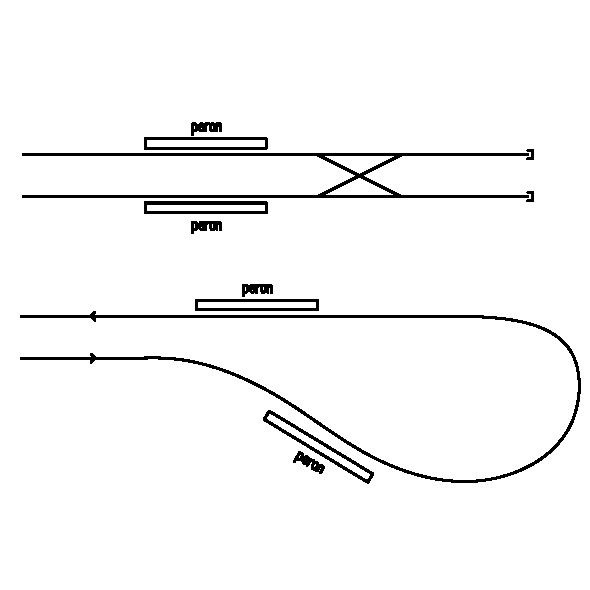
\includegraphics[trim={0 1cm 0 1cm},clip,scale=1]{uklady.pdf}\\
		\label{uklady}
		
		\footnotesize{źródło: opracowanie własne}
	\end{figure}
	
	Pętle tramwajowe stosowane są w znacznej większości przypadków. Podstawowe typy można podzielić ze względu na kilka różnych czynników. Ze względu na położenie w trasie linii tramwajowej pętle mogą być końcowe oraz pośrednie. Schematy takich pętli pokazano na rysunku \ref{petle1}.
	
	\begin{figure}[H]
	\centering
	\caption{Podział pętli tramwajowych ze względu na położenia w trasie}
	\begin{subfigure}{.33\textwidth}
	  \centering
	  \caption{pośrednia jednokierunkowa}
	  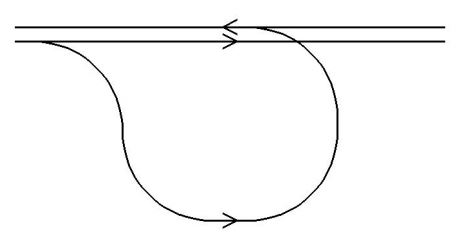
\includegraphics[width=\linewidth]{petle1}
	\end{subfigure}%
	\begin{subfigure}{.33\textwidth}
	  \centering
	  \caption{pośrednia dwukierunkowa}
	  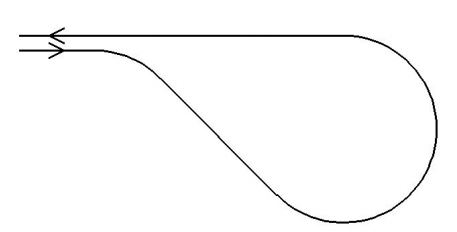
\includegraphics[width=\linewidth]{petle2}
	\end{subfigure}%
	\begin{subfigure}{.33\textwidth}
	  \centering
	  \caption{końcowa}
	  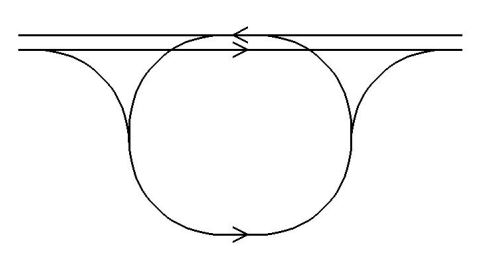
\includegraphics[width=\linewidth]{petle3}
	\end{subfigure}
	\label{petle1}\\
	\footnotesize{źródło: Makuch J., wykład w formie elektronicznej, kurs Koleje Miejskie, Politechnika Wrocławska, \url{http://www.zits.pwr.wroc.pl/makuch/kmm_W1.pdf} \cite{makuch}}
	\end{figure}

	Kształt pętli tramwajowych może być bardzo zróżnicowany i dyktowany jest najczęściej warunkami terenowymi i przestrzennymi w miejscu planowanej inwestycji. Podstawowe kształty pokazano na rysunku \ref{petle2}.
	
	\begin{figure}[H]
	\centering
	\caption{Podział pętli tramwajowych ze względu na kształt}
	\begin{subfigure}{.25\textwidth}
	  \centering
	  \caption{,,kropla'' niesymetryczna}
	  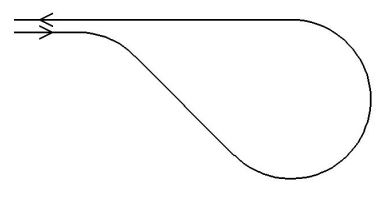
\includegraphics[width=\linewidth]{petle4}
	\end{subfigure}%
	\begin{subfigure}{.25\textwidth}
	  \centering
	  \caption{,,kropla'' symetryczna}
	  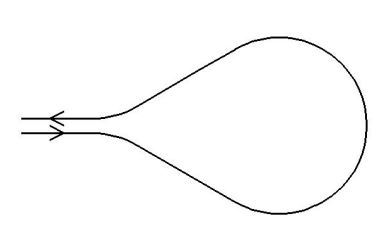
\includegraphics[width=\linewidth]{petle6}
	\end{subfigure}%
	\begin{subfigure}{.25\textwidth}
	  \centering
	  \caption{,,zerówka''}
	  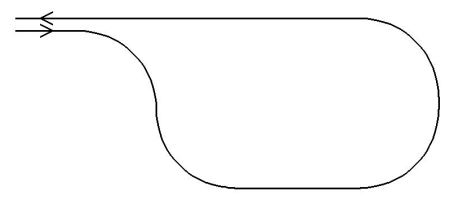
\includegraphics[width=\linewidth]{petle5}
	\end{subfigure}%
		\begin{subfigure}{.25\textwidth}
	  \centering
	  \caption{,,trójkąt''}
	  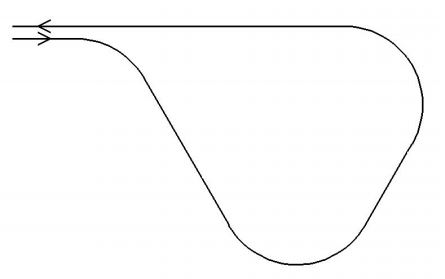
\includegraphics[width=\linewidth]{petle7}
	\end{subfigure}
	\label{petle2}\\
	\footnotesize{źródło: Makuch J., wykład w formie elektronicznej, kurs Koleje Miejskie, Politechnika Wrocławska, \url{http://www.zits.pwr.wroc.pl/makuch/kmm_W1.pdf} \cite{makuch}}
	\end{figure}
	
	Ze względu na kierunek ruchu tramwajów po pętli możemy je podzielić na pętle o ruchu normalnym (czyli prawostronnym) oraz o ruchu odwróconym (lewostronnym, zegarowym). Wybór konkretnego rozwiązania ma wpływ na lokalizację przystanków. Do taboru z drzwiami jedynie po jedne stronie pasażerowie mogą wsiadać tylko z prawej strony zatem w przypadku odwróconego układu ruchu na pętli konieczne będzie lokalizowanie przystanków wewnątrz pętli. Schematy obu rozwiązań pokazano na rysunku \ref{petle3}.
	
	\begin{figure}[H]
	\centering
	\caption{Podział pętli tramwajowych ze względu na kierunek ruchu}
	\begin{subfigure}{.33\textwidth}
	  \centering
	  \caption{układ normalny}
	  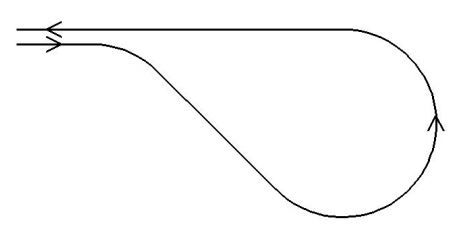
\includegraphics[width=\linewidth]{petle8}
	\end{subfigure}%
	\begin{subfigure}{.33\textwidth}
	  \centering
	  \caption{układ odwrócony}
	  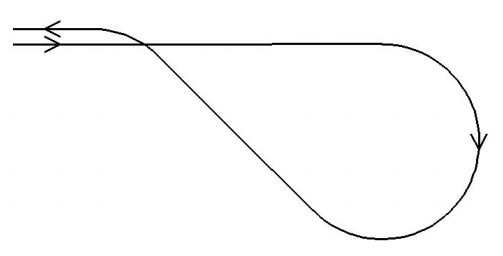
\includegraphics[width=\linewidth]{petle9}
	\end{subfigure}
	\label{petle3}\\
	\footnotesize{źródło: Makuch J., wykład w formie elektronicznej, kurs Koleje Miejskie, Politechnika Wrocławska, \url{http://www.zits.pwr.wroc.pl/makuch/kmm_W1.pdf} \cite{makuch}}
	\end{figure}
	
	Pętle tramwajowe różnią się również pod względem organizacji układu przystanków. Ponieważ przyjeżdżające na pętlę tramwaje muszą odczekać zanim ponownie wyruszą w trasę konieczne jest zapewnienie miejsca postojowego (torów postojowych). Przystanek dla wysiadających można umieścić przed torami postojowymi uzyskując wtedy schemat ,,koniec -- postój'' gdzie pasażerowie ze wszystkich linii wysiadają na tym samym przystanku -- rysunek \ref{petle4a}. Rozwiązanie takie jest bardziej korzystne dla pasażerów. Zastosowane jest m. in. na wrocławskich pętlach Biskupin, Park południowy lub Tarnogaj. Przystanki dla wysiadających można także umieścić równolegle do torów postojowych tak aby każdy tor (każda linia) miała własny przystanek końcowy (schemat ,,koniec\slash postój'', rysunek \ref{petle4b}) . Takie rozwiązanie zastosowano na przykład na pętlach Jelitkowo w Gdańsku oraz na pętli Oporów we Wrocławiu przed przebudową. 
	
	Przystanki dla wsiadających można umieścić za torami postojowymi, wtedy każda linia zaczynająca bieg na pętli będzie zabierała pasażerów z tego samego przystanku (schemat ,,postój -- start''). Jest to zalecane rozwiązanie, bo umożliwia pasażerom na wybór połączenia w zależności od czasu przyjazdu bez konieczności obserwowania kilku przystanków naraz. Zastosowano to rozwiązanie na przykład na pętlach Osobowice we Wrocławiu oraz Łostowice w Gdańsku. Przystanki dla wsiadających mogą być także umieszczone obok torów postojowych w układzie ,,postój\slash start'' -- rysunek \ref{petle4c}. Jest to schemat wyjątkowo niewygodny dla pasażerów, którzy muszą podjąć decyzję wyboru połączenia przed wejściem na przystanek lub zmuszeni są do szybkiej zmiany przystanków w przypadku zmiany zdania. Rozwiązanie takie zastosowane jest na przykład na pętlach Leśnica lub Oporów. 
	
		\begin{figure}[H]
	\centering
	\caption{Układ przystanków na pętli}
	\begin{subfigure}{.33\textwidth}
	  \centering
	  \caption{koniec -- postój -- start}
	  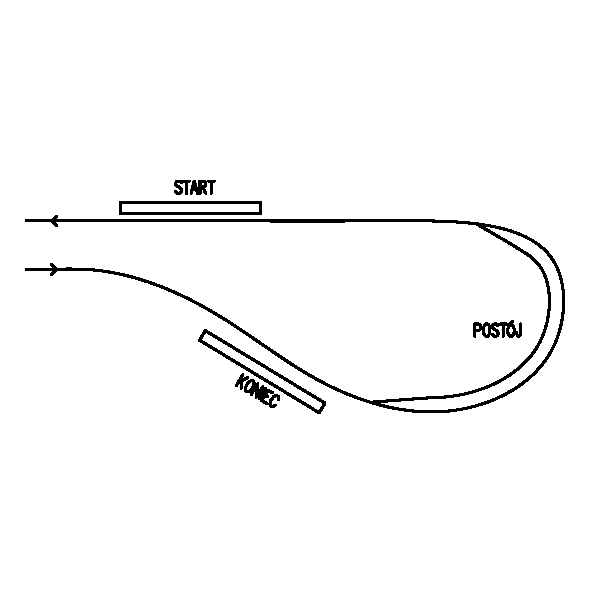
\includegraphics[clip,trim={0 2cm 0 2cm},width=\linewidth]{petle10}
	  \label{petle4a}
	\end{subfigure}%
	\begin{subfigure}{.33\textwidth}
	  \centering
	  \caption{koniec\slash postój -- start}
	  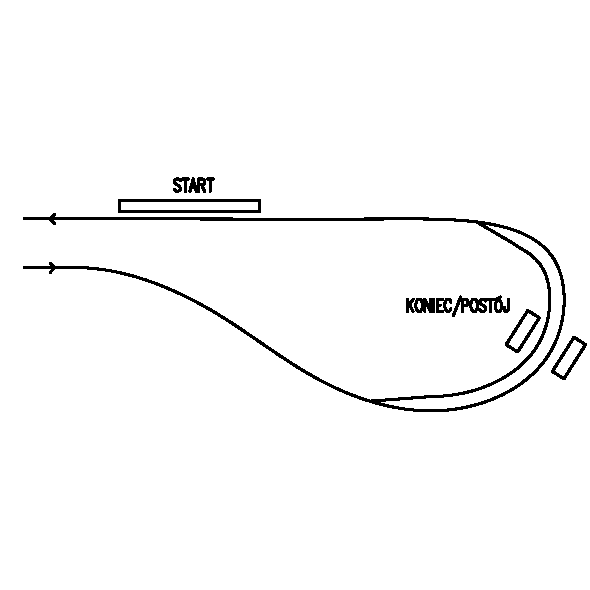
\includegraphics[clip,trim={0 2cm 0 2cm},width=\linewidth]{petle11}
	  \label{petle4b}
	\end{subfigure}%
	\begin{subfigure}{.33\textwidth}
	  \centering
	  \caption{koniec -- postój\slash start}
	  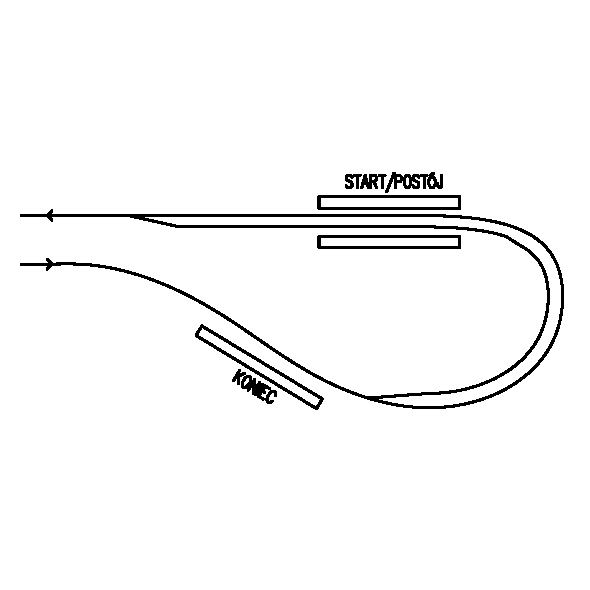
\includegraphics[clip,trim={0 2cm 0 2cm},width=\linewidth]{petle12}
	  \label{petle4c}
	\end{subfigure}
	
	\footnotesize{źródło: opracowanie własne}
	\end{figure}
	
	\clearpage
	\subsection{Ciągi piesze i rowerowe} \label{sec:ciagi_piesze}
	
	\subsubsection{Zalecenia ogólne}
	
	Najważniejszym użytkownikiem węzła przesiadkowego jest pieszy i to jemu powinien być podporządkowany układ dworca. Dokładna analiza ruchu pieszych pozwala na określenie wymaganych szerokości chodników, ewentualnych schodów, ramp oraz usytuowanie i szerokość peronów. Układ chodników i ścieżek powinien być maksymalnie czytelny dla pieszego, tj. prostoliniowy i intuicyjny. Wszelkie przecięcia z jezdnią powinny być pokonywane prostopadle oraz należy unikać zmian poziomu czyli schodów, ramp i przejść podziemnych lub nadziemnych  \cite{zaluski}. Cały układ powinien być zwarty architektonicznie i przemyślany, aby nie było w nim punktów, z których nikt nie korzysta oraz punktów nadmiernie zatłoczonych. Aby całość była atrakcyjna wizualnie i użytkowo należy pamiętać o odpowiedniej liczbie ławek, wiat, koszy na śmieci oraz tablic informacyjnych. 
	
	Jeśli chodzi o ciągi piesze w ujęciu osób niepełnosprawnych należy stosować jak najmniejszą liczbę schodów oraz ostrych podejść. Wszelkie konieczne zmiany poziomów powinny się odbywać za pomocą łagodnych pochylni (o maksymalnie kilkuprocentowym spadku). Korzystając z doświadczeń płynących z istniejących węzłów przesiadkowych, należy unikać stosowania podnośników przyschodowych dla osób niepełosprawnych. Są one praktycznie nieużytkowane, nie spełniają swoich funkcji i dodatkowo są przeszkodą dla osób korzystających ze schodów \cite{zaluski}. 
	
	Dobrym przykładem trzymania się tych zasad jest zintegrowany dworzec przesiadkowy w Tczewie (kolej+autobus), którego rzut pokazany jest na rysunku \ref{tczew}. Różnica poziomów pomiędzy częścią autobusową a dojściem do dworca PKP wynosi prawie 4 metry i jest realizowana przez rampę o stałym pochyleniu dzięki czemu cały obiekt jest bezproblemowo dostępny również dla osób niepełnosprawnych. Kosztem utrzymania niedużych różnic poziomów jest konieczność poprowadzenia drogi dojazdowej tunelem pod ciągiem pieszym. Jest to rozwiązanie droższe ale bardzo komfortowe dla pieszych.
	
	\begin{figure}[H]
		\centering
		\caption{Rzut zintegrowanego węzła przesiadkowego w Tczewie}
		\includegraphics[width=\linewidth]{tczew}\\
		\footnotesize{źródło: Załuski D., \emph{Zintegrowane węzły przesiadkowe przy małych dworcach kolejowych}, ,,TTS Technika Transportu Szynowego'' str. 62--68, nr 21, 2014. \cite{zaluski}}
		\label{tczew}
	\end{figure}
	
	\begin{samepage}Przy projektowaniu ciągów pieszych należy szczególnie zwrócić uwagę na szerokości chodników aby zapewnić komfort użytkowania. Rozporządzenie Ministra Transportu i Gospodarki Morskiej z dnia 02.03.1999r. w sprawie warunków technicznych, jakim powinny odpowiadać drogi publiczne i ich usytuowanie (Dz. U. z 1999r. nr 43, poz. 430)  podaje minimalne szerokości chodników jako: 
	\begin{quote}
	§44.4 Szerokość chodnika odsuniętego od jezdni lub szerokość samodzielnego ciągu pieszego nie powinna być mniejsza niż 1,5 m, a dopuszcza się miejscowe zmniejszenie szerokości chodnika do 1,0 m, jeżeli jest on przeznaczony wyłącznie do ruchu pieszych \cite{rozporzadzenie_drogi}
\end{quote}
	 oraz w punkcie 5: 
\begin{quote}
	 §44.5 Długość chodnika usytuowanego w ciągu przejść dla pieszych między jezdniami lub między jezdnią a torowiskiem tramwajowym powinna wynosić nie mniej niż 2,0 m \cite{rozporzadzenie_drogi}
	 \end{quote}\end{samepage}
	 
	 W innych krajach wartości te są podobne. W Anglii nie ma prawnie określonych minimalnych wartości szerokości chodników, ale są one zalecane m. in. w poradnikach projektowania dróg jako dwa metry \cite{young}. W USA minimalna wartość zalecana wynosi 6 stóp, czyli około 1,8 metra \cite{guidelines_washington}. 
	 
	 Warto nadmienić, że jest to szerokość minimalna. W przypadku węzłów przesiadkowych ruch pieszych jest wzmożony, liczba pieszych uzależniona jest od wielkości węzła i liczby połączonych z nim linii. Poza tym, ruch pieszych jest mniej płynny niż w przypadku chodników przydrogowych -- piesi spieszą się do pracy, często niosą torby i walizki, a wielu z nich dobiega do przystanków aby zdążyć na odjeżdżający tramwaj lub autobus. Dodatkowym faktem jest nierównomierne rozłożenie ruchu pieszych w czasie. Liczba użytkowników chodnika zwiększa się w okresach przyjazdu i odjazdu pojazdów komunikacji zbiorowej. Biorąc pod uwagę te fakty, konieczne jest zatem zastosowanie szerszych chodników (niż postulowane dwa metry) na terenie węzłów przesiadkowych. 
	 
	 \subsubsection{Poziom swobody ruchu pieszych}
	 
	 Wyznaczenie szerokości minimalnej aby ruch pieszych był płynny zależne jest od natężenia ruchu pieszych, motywacji pieszych i ich cech indywidualnych oraz od oczekiwanego poziomu swobody ruchu. Prędkość poruszania się pieszych zależna jest od celu podróży oraz ieku i płci. Do obliczeń ruchu na obszarze węzła przesiadkowego można przyjąć prędkość $V_p = 1.49 \ \si{km/h}$. Przepustowość ruchu pieszych na chodniku określa się jako liczbę pieszych w czasie wg wzoru \cite{standardy_wroclaw}:
	 \begin{equation}
	 C_p = \frac{L_p}{t}
	 \end{equation}
	 Liczbę pieszych można obliczyć ze wzoru \cite{standardy_wroclaw}:
	 \begin{equation}
	 L_p = k \cdot V_p \cdot B \cdot t
	 \end{equation}
	 Gdzie $k$ -- gęstość ruchu pieszego (os/m2), $V_p$ -- prędkość pieszych (m/s), $B$ -- efektywna szerokość przekroju urządzenia dla pieszych (m), $t$ -- okres czasu (s). 
	 Dla ustalenia przepustowości należy ustalić gęstość i prędkość ruchu pieszych \cite{standardy_wroclaw}:
	 \begin{equation}
	 k=\frac{Q_p}{V_p}
	 \end{equation}
	 Poziomy swobody ruchu pieszych, tak jak dla ruchu samochodowego, są oznaczone literami alfabetu gdzie poziom A oznacza największą swobodę ruchu. Wszystkie poziomy pokazane są w tabeli \ref{psr_piesi}.
	 % Table generated by Excel2LaTeX from sheet 'Sheet2'
\begin{table}[H]
  \centering
  \caption{Poziomy swobody ruchu pieszych}
    \begin{tabular}{p{1cm}p{3cm}p{2cm}p{8cm}}
    \hline
    PSR & Pow. na 1 osob [m2/os] & Gęstość $k$ [os/m2] & Warunki ruchu \bigstrut[b]\\
    \hline
    A          & $\geq 5.5$  & $0 \div 0.1$ & Swoboda poruszania się, brak konieczności zmiany toru ruchu \bigstrut[t]\\
    B          & $3.7 \div 5.5$ & $0.1 \div 0.25$ & Sporadyczna konieczność zmiany toru ruchu \\
    C          & $2.2 \div 3.7$ & $0.24 \div 0.4$ & Częsta konieczność zmiany toru ruchu \\
    D          & $1.4 \div 2.2$ & $0.4 \div 0.7$ & Ograniczenie prędkości poruszania oraz możliwość wyprzedzania wolniejszych pieszych \\
    E          & $0.8 \div 1.4$ & $0.7 \div 1.8$ & Ograniczenie prędkości poruszania, przy bardzo ograniczonej możliwości wyprzedzania wolniejszych pieszych \\
    F          & $\leq 0.8$ & $\geq 1.8$ & Bardzo duże ograniczenie prędkości poruszania, częsty kontakt z innymi pieszymi \\
    \hline
    & & & \\
    \end{tabular}%
  \label{psr_piesi}
  
  \zrodlo{źródło: Bocheńska-Niemiec A., Cebrat K., Kusowska K., Romanik A., Tyrka Ł., Walter E., Wiszniowski J., \emph{Wrocławskie standardy kształtowania przestrzeni miejskich przyjaznych pieszym}, Gmina Wrocław, maj 2017 \cite{standardy_wroclaw}}
\end{table}%

	 
	 \subsubsection{Wytyczne dla miasta Wrocław}
	 
	 Aby zapewnić komfort poruszania się pieszych i rowerzystów należy stosować odpowiednie nawierzchnie chodników i dróg rowerowych. We Wrocławiu zalecane jest stosowanie siedmiu podstawowych rodzajów nawierzchni wyszczególnionych w Katalogu Standardów Nawierzchni Chodników dla Wrocławia \cite{standardy_chodnik}.

\begin{samepage}
Nawierzchnie chodników na obszarze staromiejskim:
	 \begin{itemize}\setlength{\itemsep}{0em}
	 \item Typ A/1 -- Chodnik z płyt kamiennych nowych w połączeniu z kostką granitową nową (stosuje się obowiązkowo w obszarze centralnym oraz gdy wymagają tego zalecenia konserwatorskie, zalecane w obszarze śródmiejskim) \cite{standardy_wroclaw}
	 \item Typ A/2 -- Chodnik z płyt kamiennych nowych w połączeniu z kostką staroużyteczną (stosuje się tak jak typ A/1) \cite{standardy_wroclaw}
	 \item Typ B -- Chodniki/place z płyt kamiennych 50x50x7
	 \item Typ C -- Chodniki z płyt kamiennych staroużytecznych w połączeniu z kostką granitową (stosuje się tak jak typ A/1) \cite{standardy_wroclaw}
	 \end{itemize}\end{samepage}
	 
	 \begin{samepage}
Nawierzchnie chodników poza obszarem staromiejskim:
	 \begin{itemize}\setlength{\itemsep}{0em}
	 \item Typ D -- Chodniki z płyt betonowych 50x50x7, 35x35x5 (rodzaj nawierzchni zalecany w przypadku, gdy chodnik nie przylega bezpośrednio do jezdni, czy linii zabudowy, poza obszarem śródmiejskim) \cite{standardy_wroclaw}
	 \item Typ E -- Chodniki z płyt betonowych 50x50 z opaską z kostki betonowej (stosowana w obszarach, w których chodnik przylega bezpośrednio do jezdni i/lub zabudowy wielorodzinnej (sytuacja występująca najczęściej w strefie śródmiejskiej) oraz na ulicach z dużą ilością naziemnej infrastruktury technicznej) \cite{standardy_wroclaw}
	 \item Typ F -- Chodniki z kostki betonowej bez faz (alternatywa dla nawierzchni z płyt betonowych, na ulicach układu podstawowego i uzupełniającego; poza obszarem centralnym i śródmiejskim, stosowanie nawierzchni z kostki betonowej i kamiennej dopuszcza się na:
zjazdach, ale tylko w miejscach, w których wjazd nie jest przecięty przez ciąg pieszy albo rowerowy -- pasy te mają zachowywać ciągłość nawierzchni; częściach chodnika przylegających do jezdni, na których dopuszczony jest postój pojazdów; ostrych łukach poziomych chodników oraz całych odcinkach chodników o dużej krętości) \cite{standardy_wroclaw}
	 \end{itemize}\end{samepage}
	 
	 Są to nawierzchnie typu kostkowego, jednak dopuszcza się także stosowanie nawierzchni typu ciągłego.
	 
	 \begin{itemize}\setlength{\itemsep}{0em}
	 \item Ciągi z nawierzchnią bitumiczną --  stosowana na obszarze całego miasta, przeznaczona wyłącznie dla ścieżek rowerowych i ciągów pieszo-rowerowych. Należy unikać wyznaczania wspólnych ciągów dla pieszych i rowerzystów, o nawierzchni bitumicznej, na obszarach centrum i śródmieścia. Zalecany obszar stosowania: tereny rekreacyjne - jako podstawowy rodzaj nawierzchni na ciągach pieszo-rowerowych;  obszary peryferyjne, charakteryzujące się niewielkim ruchem pieszym i rowerowym; ciągi pieszo-rowerowe, przebiegające w oddaleniu od zabudowań, z przewagą ruchu rowerowego.  Zaleca się unikać lokalizacji sieci podziemnych pod ciągami o nawierzchni bitumicznej \cite{standardy_wroclaw}. 
	\item Chodnik o nawierzchni z kruszywa mineralnego -- rekomendowany dla ciągów pieszych i pieszo-rowerowych o niewielkim natężeniu ruchu, na terenach rekreacji i miejskich skwerach \cite{standardy_wroclaw}.
	\item Chodnik o nawierzchni z mieszanki żywiczno-mineralnej -- Zalecane stosowanie w miejscach, z których trudno jest odprowadzić wodę opadową: tereny rekreacyjne, zwłaszcza główne ciągi piesze i rowerowe - o dużym natężeniu ruchu;  miejskie skwery, place zabaw, boiska; obszary i pasy pozakomunikacyjne, w przekroju ulicy, przeznaczone na strefy aktywności społecznych; otoczenie drzew sadzonych w pasach bocznych chodników. Odradza się lokalizowania sieci podziemnych pod ciągami o nawierzchni mineralno-żywicznej \cite{standardy_wroclaw}. 
	 \end{itemize}
	 
	 \subsection{Obsługa osób niepełnosprawnych oraz starszych}
	 
	 Ze względu na to, że osoby starsze i niepełnosprawne często nie są w stanie samodzielnie korzystać z samochodów lub sprawia im to duży problem, decydują się one w dużej mierze na korzystanie z komunikacji publicznej. Konieczne jest zatem dostosowanie infrastruktury publicznej do specyficznych wymagań, tak aby osoby te mogły komfortowo korzystać z komunikacji zbiorowej oferowanej przez miasto. Dotyczy to także węzłów przesiadkowych.
	 
	 W skład udogodnień służących poprawie komfortu użytkowania przez osoby z ograniczonymi możliwościami ruchowymi zalicza się wiele urządzeń oraz rozwiązań architektoniczno-budowlanych, które powinny być uwzględnione już na etapie projektowania węzła przesiadkowego. Są to m. in. urządzenia do obsługi osób niepełnosprawnych (chodniki ruchome, schody ruchome, dźwigi osobowe i podnośniki przyschodowe), obiekty budowlane takie jak rampy i pochylnie dla osób niepełnosprawnych, a także odpowiednie rozwiązania budowlane jak minimalizacja różnic poziomów koniecznych do pokonania, odpowiednie wysokości i szerokości schodów, stopni, progów i uskoków, minimalizacja odległości pomiędzy elementami węzła i zastosowanie odpowiedniej szerokości ciągów pieszych \cite{poznan}.
	 
	 Pochylnie są zalecaną formą realizacji różnicy poziomów w przypadku osób niepełnosprawnych. Są niezawodne i tanie w utrzymaniu, choć zajmują więcej miejsca niż dźwigi osobowe. Wymiary pochylni przeznaczonych dla osób niepełnosprawnych określa Rozporządzenie Ministra Infrastruktury z dnia 12 kwietnia 2002 r.	w sprawie warunków technicznych, jakim powinny odpowiadać budynki i ich usytuowanie w paragrafie §71 \cite{warunki_techniczne}:
	 \begin{quote}
	 § 71. 1. Pochylnie przeznaczone dla osób niepełnosprawnych powinny mieć szerokość płaszczyzny ruchu 1,2 m, krawężniki o wysokości co najmniej 0,07 m i obustronne poręcze odpowiadające warunkom określonym w § 298, przy czym odstęp między nimi powinien mieścić się w granicach od 1 m do 1,1 m.
	 
2. Długość poziomej płaszczyzny ruchu na początku i na końcu pochylni powinna wynosić co najmniej 1,5 m.

3. Powierzchnia spocznika przy pochylni dla osób niepełnosprawnych poruszających się na wózkach inwalidzkich powinna mieć wymiary co najmniej 1,5 x 1,5 m poza polem otwierania skrzydła drzwi wejściowych do budynku.

4. Krawędzie stopni schodów w budynkach mieszkalnych wielorodzinnych i użyteczności publicznej powinny wyróżniać się kolorem kontrastującym z kolorem posadzki.
	 \end{quote}
	 
	 Zaś pochylenia dopuszczalne przez przepisy  w paragrafie §70 w postaci tabeli, którą pokazano w tabeli \ref{pochylnie}.
	 	\begin{table}[H]
		\centering
		\caption{Maksymalne nachylenie pochylni}
		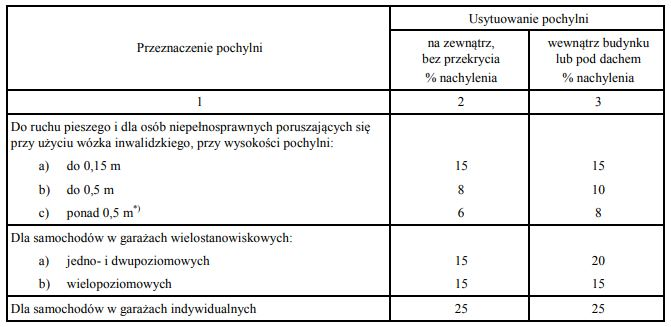
\includegraphics[width=\linewidth]{pochylnie.png}\\
		\footnotesize{źródło: Rozporządzenie Ministra Infrastruktury z dnia 12 kwietnia 2002 r.	w sprawie warunków technicznych, jakim powinny odpowiadać budynki i ich usytuowanie \cite{warunki_techniczne}}
		\label{pochylnie}
	\end{table}
	
	Stosowanie dźwigów osobowych (wind) i podnośników przyschodowych jest odradzane z uwagi na dużą awaryjność tych urządzeń i wysokie koszty eksploatacji. Podobnie jest w przypadku schodów i chodników ruchomych. Nie jest możliwe zastosowanie ich na zewnątrz a ich wykorzystanie przez osoby niepełnosprawne jest bardzo mała. 
	
	Duże znaczenie dla osób niepełnosprawnych ma odpowiednia infrastruktura peronów autobusowych i tramwajowych. Nawierzchnia peronów powinna być pokryta materiałem antypoślizgowym oraz wyposażona w płytki ostrzegawcze z wypustkami przy krawędziach. Nawierzchnie chodników i innych ciągów pieszych powinny być wyposażone w specjalne płyty kierujące dla osób niewidomych lub niedowidzących. Wysokość peronów powinna być tak dobrana aby zminimalizować różnicę poziomów pomiędzy peronem a pojazdem komunikacji. Dzięki takiemu rozwiązaniu przejazd wózkiem lub wejście osoby starszej do pojazdu będzie komfortowe.
	
	Wszystkie urządzenia służące osobom niepełnosprawnym powinny być specjalnie oznaczone za pomocą odpowiednich piktogramów. Na terenie węzła należy także rozważyć stosowanie powierzchni malowanych informujących o niebezpieczeństwach na przykład w pobliżu peronów. Przejścia dla pieszych powinny być dobrze widoczne i, w przypadku przejść z sygnalizacją, wyposażone w system nadawania sygnałów dźwiękowych. 
	 
	 
\subsection{Przystanki autobusowe i tramwajowe}

	Przystanki są newralgicznym punktem węzła przesiadkowego. Właściwa ich lokalizacja i odpowiednie zaprojektowanie podnosi atrakcyjność węzła dla podróżnych. Jeśli jest taka możliwość należy dążyć do integracji przystanków różnych linii i rodzajów transportu aby zwiększyć komfort przesiadek. W przypadku obecności dużej liczby linii należy lokalizować perony obok siebie w taki sposób aby uzyskać najkrótszy czas przejścia między peronami. Zintegrowane przystanki powinny być połączone przejściami po obu stronach (na końcu i na oczątku) \cite{standardy_wroclaw}. 
	
	\subsubsection{Wymiary zatok i przystanków}

	%\begin{samepage}
	Wymiary i usytuowanie zatok autobusowych określa Rozporządzenie Ministra Transportu i Gospodarki Morskiej w sprawie warunków technicznych, jakim powinny odpowiadać drogi publiczne i ich usytuowanie \cite{rozporzadzenie_drogi}. Wymogi te podane są w §119., zaś szczegółowe wymiary są następujące:
	\begin{quote}
	§119.8. Zatoka autobusowa powinna być wykonana, z zastrzeżeniem ust. 9, o parametrach nie mniejszych niż: \\
1)	długość krawędzi zatrzymania - 20,0 m; \\
2)	szerokość zatoki przy jezdni - 3,0 m; \\
3)	szerokość zatoki - 3,5 m, jeżeli jest ona oddzielona od jezdni bocznym pasem dzielącym; \\
4)	wyokrąglenie załomów krawędzi jezdni łukami o promieniu - 30,0 m; \\
5)	szerokość peronu - 1,5 m; \\
6)	pochylenie poprzeczne jezdni w zatoce 2,0\%, skierowane do krawędzi jezdni drogi lub zgodnie z jej pochyleniem, w zależności od warunków odwodnienia. \\
Skos wyjazdowy z drogi nie powinien być większy niż 1 : 8, a skos wjazdowy na drogę nie większy niż 1 : 4. \\
	\end{quote}%\end{samepage}
	
	\subsubsection{Wyposażenie przystanków}
	
	Wszystkie przystanki należy wyposażyć w minimum słup przystankowy wraz z rozkładem, kosz na śmieci oraz wiatę przystankową. Przystanki, które obsługują dużą liczbę pasażerów powinny ponadto posiadać ławki i powiększone wiaty. Podstawowym typem wiaty stosowanym we Wrocławiu jest konstrukcja stalowa o głębokości 1,5 metra oraz szerokości czterech segmentów po 1,4 metra każdy (5,6 metra łącznie), przy czym na przystankach o niskim natężeniu ruchu można zastosować wiatę o jedynie trzech segmentach \cite{standardy_wroclaw}. Przykładowa wiata pokazana jest na rysunku \ref{przystanek_wiata}. Dodatkowo, należy zapewnić pas minimum 2,5 metra od krawędzi wiaty do krawędzi peronu autobusowego. Jeśli jest to niemożliwe należy zastosować węższe wiaty. 
	
		\begin{figure}[H]
		\centering
		\caption{Standardowa wiata przystankowa stosowana we Wrocławiu}
		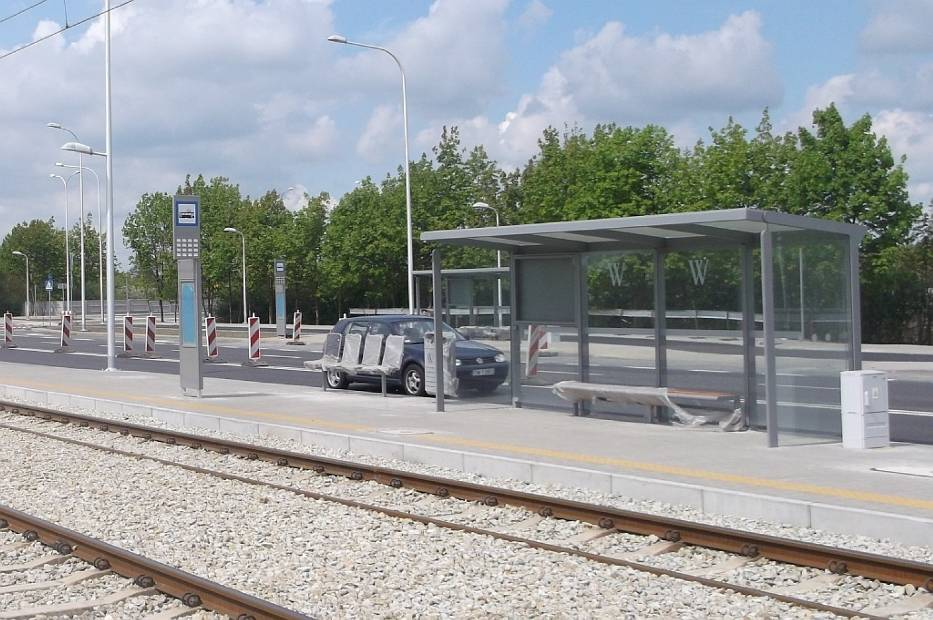
\includegraphics[width=0.75\linewidth]{przystanek_wiata}\\
		\footnotesize{źródło: \url{http://wroclaw.naszemiasto.pl}}
		\label{przystanek_wiata}
	\end{figure}
	
	\subsection{Pętle tramwajowe}
	
	\section{Studia istniejących rozwiązań}
	
	\clearpage
	\subsection{Pętla Łostowice-Świętokrzyska, Gdańsk}
	
	Węzeł tramwajowo-autobusowy Łostowice-Świętokrzyska został oficjalnie otwarty 11 maja 2012 roku, a pierwsze połączenia ruszyły dzień później 12 maja \cite{gazeta_gdansk}. Znajduje się on w dzielnicy Chełm przy skrzyżowaniu ulicy Świętokrzyskiej i alei Vaclava Havla. W inwestycji razem z pętlą został wykonany odcinek trasy tramwajowej w ciągu ulicy Świętokrzyskiej. Lokalizację węzła w odniesieniu do układu tramwajowego miasta pokazano na rysunku \ref{lostowice1}.
	
	\begin{figure}[H]
		\centering
		\caption{Lokalizacja węzła Łostowice-Świętokrzyska (Gdańsk)}
		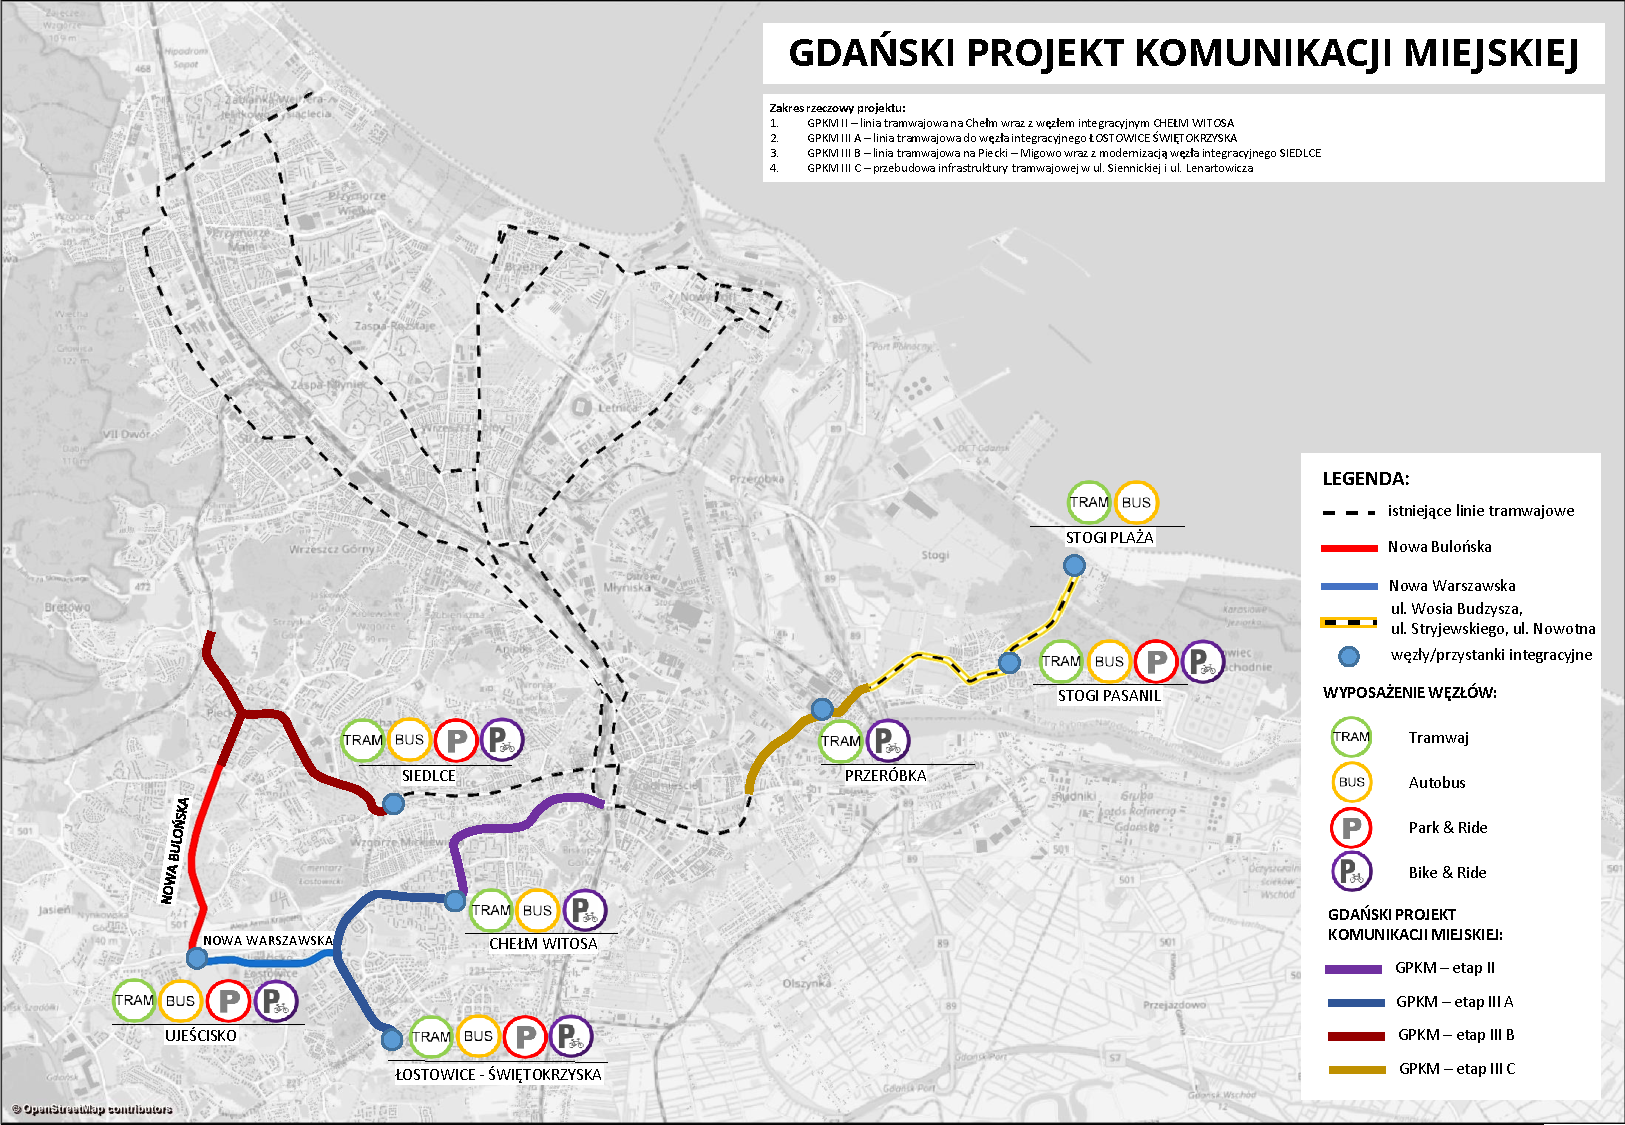
\includegraphics[width=1\linewidth]{Lostowice/edroga_pl.pdf}\\
		\footnotesize{źródło: \url{https://www.edroga.pl}}
		\label{lostowice1}
	\end{figure}
	
	Budowa linii tramwajowej wraz z pętlą była realizowana przez spółkę miejską Gdańskie Inwestycje Komunalne i trwała od listopada 2010 roku do maja 2012. Budowa ta była częścią wykonaną w ramach programu inwestycyjnego -- Gdańskiego Projektu Komunikacji Miejskiej (GPKM) etap III A. Jest to projekt rozwoju gospodarczo-społecznego regionu pomorskiego, którego głównym beneficjentem było miasto Gdańsk. Wartość projektu to 667 mln złotych, z czego około 408 mln zostało dofinansowane ze środków Europejskiego Funduszu Spójności (Program Infrastruktura i Środowisko). Wykonawcą inwestycji było konsorcjum dwóch firm: Firma Budowlano-Drogowa MTM S.A. oraz Trakcja Polska S.A. \cite{portal_gdansk}. 
	
	\begin{samepage}
	W ramach całego podetapu GPKM zrealizowano \cite{portal_gdansk}:
	\begin{itemize}\setlength{\itemsep}{0em}
	\item wydłużenie linii tramwajowej z dzielnicy Chełm do nowej pętli tramwajowej na skrzyżowaniu al. Havla i ul. Świętokrzyskiej w dzielnicy Gdańsk Południe, która przebiega ul. Witosa i al. Havla, odcinek o długości 3,35 km
	\item modernizację 12 odcinków istniejących torowisk, o łącznej długości 12,06 km
	\item budowę i przebudowę urządzeń elektroenergetycznych zasilających trakcję tramwajową
	\item przebudowę zajezdni tramwajowej Wrzeszcz
	\item zakup taboru tramwajowego – 35 nowoczesnych składów tramwajowych firmy PESA
	\item wybudowanie omawianej pętli autobusowo-tramwajowej.
	\end{itemize}\end{samepage}
	
	Konieczność przeprowadzenia inwestycji budowy nowej linii tramwajowej i pętli Łostowice-Świętokrzyska wynikała z bardzo szybkiego rozwoju dzielnicy Chełm. Jest to dzielnica, która w latach 1998-2006, charakteryzowała się jednym z największych wskaźników zmiany liczby mieszkańców -- z 43 tys. w roku 1998 do 52 tys. w roku 2006, co stanowiło wzrost o ok. 20\% \cite{opracowanie_gdansk}. Pomimo tak dużej liczby mieszkańców brak było bezpośredniego połączenia tramwajowego z centrum miasta.
	
	Gdańsk jest miastem o problematycznym układzie drogowym. Ze względu na niekorzystne ukształtowanie terenu -- wzgórza morenowe -- liczba dróg pozwalająca na dojazd z i do zachodnich i południowych części miasta jest niewystarczająca. Powoduje to duże zatłoczenie istniejących tras. Z tego powodu konieczne było lepsze połączenie tych rejonów z komunikacją publiczną, w szczególności tramwajową, gdyż analiza pokazuje, że mieszkańcy preferują korzystanie ze środków transportu indywidualnego w przypadku gdy dostępna jest jedynie alternatywa autobusowa. Dostępne połączenia autobusowe, które dojeżdżały do okolic nieistniejącego jeszcze węzła przez ulicę Łódzką (obecnie: aleja Vaclava Havla) obsługiwały nawet po 11 tysięcy pasażerów dziennie, co pokazane jest na rysunku \ref{lostowice2}, który powstał na podstawie obliczeń wykonanych po etapie II GPKM w roku 2008. Biorąc pod uwagę dynamiczny wzrost liczby mieszkańców omawianego rejonu uznano za konieczne dostarczenie alternatywy dla połączeń autobusowych, w postaci nowej trasy tramwajowej, która jak przyjęto, miała przejąć aż do 85\% obecnego wówczas potoku obsługiwanego przez autobusy.
	
	\begin{figure}[H]
		\centering
		\caption{Natężenie ruchu autobusowego w okolicach węzła Łostowice-Świętokrzyska}
		\includegraphics[width=0.75\linewidth]{Lostowice/1}\\
		\footnotesize{źródło: Mordak R., WYG International Sp. z o.o., \emph{Studium wykonalności dla zadań inwestycyjnych i 
		modernizacyjnych przewidzianych do realizacji w latach 2008-2011}, Gdański Projekt Komunikacji Miejskiej etap IIIa, 
		Warszawa, listopad 2008. \cite{opracowanie_gdansk}}
		\label{lostowice2}
	\end{figure}
	
	Węzeł ten niewątpliwie okazał się sukcesem pomimo początkowych problemów związanych m. in. z wykonastwem -- występujące znaczne odkształcenia szyn poodowały duże opóźnienia, oraz z organizacją ruchu -- niewystarczający priorytet tramwajów \cite{kaszubowski}. Badania wykazały, że 86\% osób ankietowanych korzystających w codziennych podróżach z tego węzła jest zadowolonych z jego funkcjonowania. Aż 89\% ankietowanych uważa, że po jego wybudowaniu podróżuje się lepiej, niż przed jego powstaniem \cite{maciej_lada}. Zdecydowana większość korzystających z węzła to piesi (70\% pasażerów) -- wynika to z bardzo dobrego położenia węzła w gęsto zabudowanej dzielnicy. Parking w systemie ,,Park and Ride'' jest znacznie mniej atrakcyjny -- jego średnie wykorzystanie to zaledwie 35\% \cite{kaszubowski}. W chwili obecnej do pętli dojeżdżają cztery linie (2, 4, 6, 7) z częstotliwością kursowania co 10 $\div$ 20 minut. 
	
	Zaprojektowana pętla przy skrzyżowaniu alei Vaclava Havela i ulicy Świętokrzyskiej ma kształt trójkątny, o ruchu tramwajów zgodnie z ruchem wskazówek zegara oraz ruchem autobusów przeciwnie do ruchu wskazówek zegara. Jej schemat przedstawiono na rysunku \ref{lostowice3}. Węzeł ten składa się z:
	\begin{itemize}\setlength{\itemsep}{0em}
	\item części przyjazdowej, wyposażonej w dwa tory, przy czym tor wewnętrzny pozwala na przesiadkę ,,drzwi w drzwi'' z komunikacją autobusową
	\item części odjazdowej, wyposażonej w jeden tor z peronem również pozwalającym  na przesiadkę w trybie ,,drzwi w drzwi''
	\item parking samochodowy z 180 miejscami postojowymi
	\item parking rowerowy z 200 miejscami postojowymi
	\item drugi, oddalony parking samochodowy
	\item pętli autobusowej pozwalającej na postój do 8 standardowych 12-metrowych autobusów
	\item punktu sprzedaży biletów wraz z toaletą
	\end{itemize}
	
	Przystanek tramwajowy dla wysiadających znajduje się w części wschodnio-północnej a dla wsiadających w części południowej węzła. Obok nich znajdują się przystanki autobusowe przy czym autobusy odjeżdżające z przystanku południowego zatrzymują się drugi raz na przystanku północno-wschodnim co pozwala pasażerom na wygodne oczekiwanie bez ryzyka ominięcia pojazdu. 
	
	\begin{figure}[H]
		\centering
		\caption{Schemat węzła Łostowice-Świętokrzyska}
		\includegraphics[clip,trim={0 0 0 2cm},width=1\linewidth]{Lostowice/2}\\
		\footnotesize{źródło: Zarząd Transportu Miejskiego w Gdańsku \url{www.ztm.gda.pl}}
		\label{lostowice3}
	\end{figure}
	
	Największym atutem omawianego węzła jest jego układ geometryczny. Korzystając z możliwości jaką była jednoczesna przebudowa najbliższego skrzyżowania rozsunięto drogi wlotowe i wylotowe dla autobusów a całą pętlę autobusową wpisano w pętlę tramwajową. Z racji, że ruch tramwajowy i autobusowy jest realizowany w przeciwnych kierunkach możliwe było zastosowanie przystanków typu ,,drzwi w drzwi'' zapewniających wysoki komfort przesiadek. W przestrzeń pośrodku pętli autobusowej wpisano parking ,,Park and Ride'' a na zewnątrz, pomiędzy pętlą autobusową i tramwajową ,,Bike and Ride''. Dzięki tym zabiegom węzeł jest intuicyjny dla pasażerów a odległości konieczne do pokonania są bardzo małe. 
	
	Pasażerowie oczekujący na pojazd mają do dyspozycji szerokie wiaty osłonięte z trzech stron, wyposażone w ławki oraz rozkłady jazdy komunikacji i plan węzła, które pokazano na rysunkach \ref{lostowice5a} i \ref{lostowice5b}.
	
	\begin{figure}[H]
	\centering
	\caption{Wyposażenie wiat przystankowych}
	\begin{subfigure}{.48\textwidth}
	  \centering
	  \caption{widok na część autobusową}
	  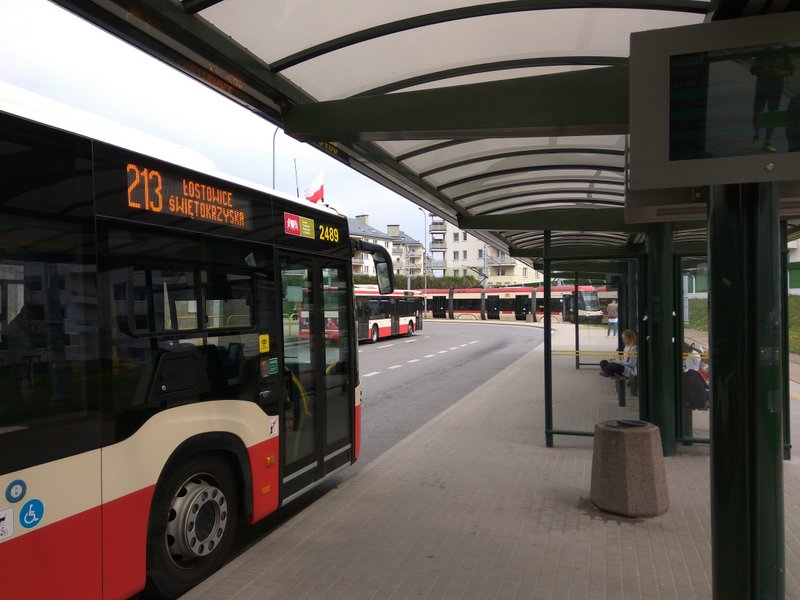
\includegraphics[width=1\linewidth]{Lostowice/moje/800px/IMG_20180501_124841}
	  \label{lostowice5a}
	\end{subfigure}%
	\hfill%
	\begin{subfigure}{.48\textwidth}
	  \centering
	  \caption{tablica informacyjna z planem węzła}
	  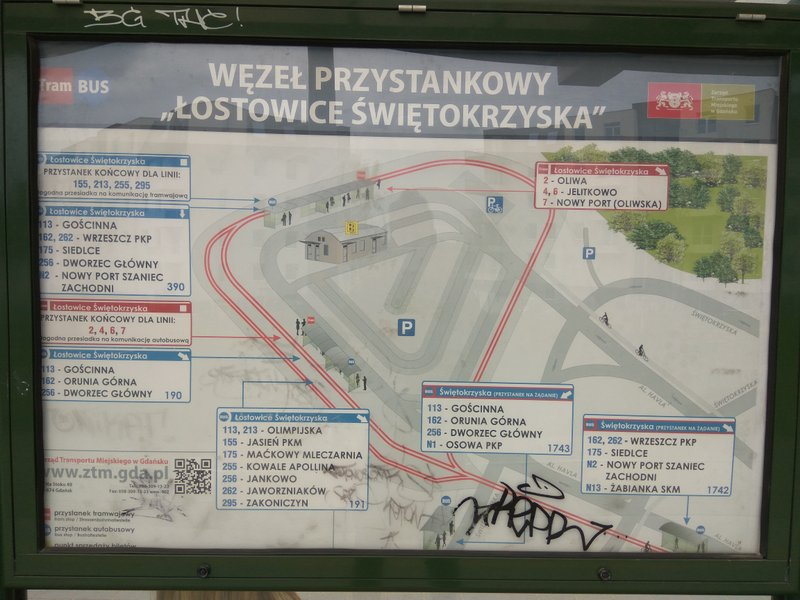
\includegraphics[width=1\linewidth]{Lostowice/moje/800px/IMG_20180501_124859}
	  \label{lostowice5b}
	\end{subfigure}
	
	\footnotesize{źródło: archiwum własne}
	\end{figure}
	
	Parking dla rowerów jest ogrodzony i wyposażony w urządzenie do napompowania opon oraz narzędzia do przeprowadzenia pomniejszych napraw.
	
	\begin{figure}[H]
		\centering
		\caption{Parking rowerowy}
		\begin{subfigure}{.66\textwidth}
	  \centering
	  \caption{widok na stojaki dla rowerów}
	  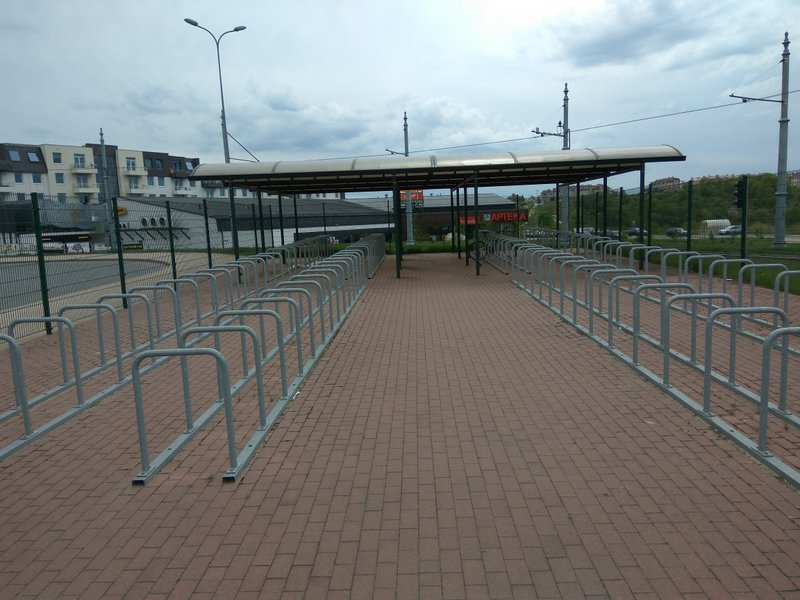
\includegraphics[scale=0.33]{Lostowice/moje/800px/IMG_20180501_124653}
		\end{subfigure}%
		\hfill%
		\begin{subfigure}{.33\textwidth}
	  \centering
	  \caption{punkt napraw}
	  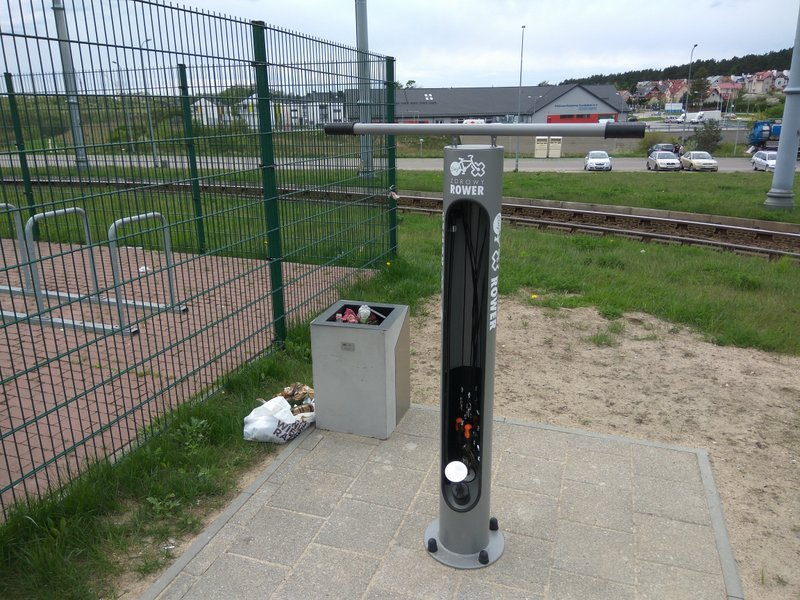
\includegraphics[clip,trim={12cm 0 0 0},scale=0.33]{Lostowice/moje/800px/IMG_20180501_124647}
		\end{subfigure}\\
		
		\footnotesize{. \\ źródło: archiwum własne}
	\end{figure}	
	
	Linie kończące bieg w omawianym węźle obsługiwane są przez tramwaje niskopodłogowe o wysokości wejścia do pojazdu równej 290 mm. Dało to możliwość zaprojektowania peronów zdecydowanie bardziej wygodnych dla pasażerów. Wysokość peronu to zaledwie 22 centymetry powyżej główki szyny. Zdjęcie peronu tramwajowego pokazano na rysunku \ref{lostowice4}.
	
		\begin{figure}[H]
		\centering
		\caption{Widok na peron tramwajowy}
		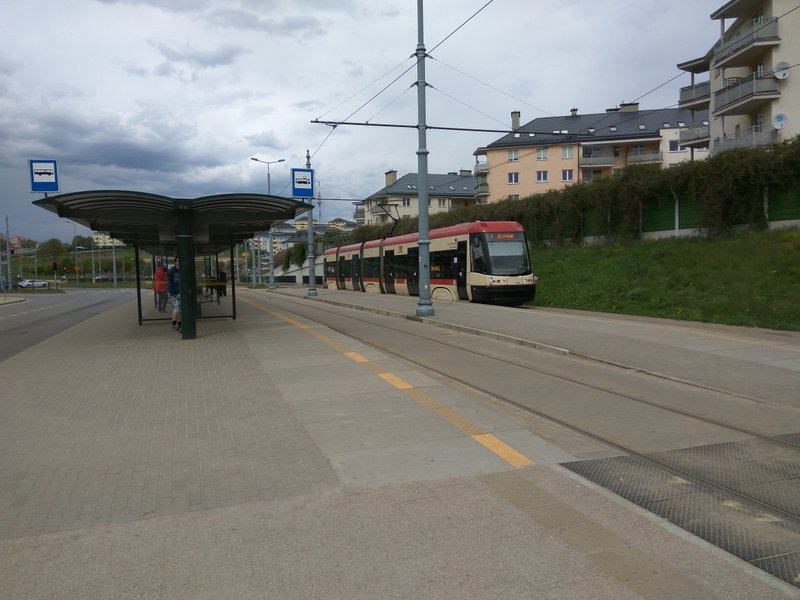
\includegraphics[width=1\linewidth]{Lostowice/moje/800px/IMG_20180501_125007}\\
		\footnotesize{źródło: archiwum własne}
		\label{lostowice4}
	\end{figure}
	
	\clearpage
	\subsection{Rondo Reagana (plac Grunwaldzki), Wrocław}
	
	Potrzebę wybudowania odpowiedniego dworca autobusowego w rejonach placu Grunwaldzkiego zauważono we Wrocławiu już w latach dziewięćdziesiątych kiedy to pojawił się pierwsze plany przebudowy problematycznego skrzyżowania ulic Piastowskiej, Marii Skłodowskiej-Curie i placu Grunwaldzkiego. Oprócz poprawienia układu samego skrzyżowania (m. in. usunięcie jednego ze wlotów) i poszerzenia głównych ulic od mostu Grunwaldzkiego do mostu Szczytnickiego postulowano także budowę dodatkowych przystanków na wylocie wszystkich głównych arterii lub budowę dworca. Pierwsze propozycje zakładały lokalizację dworca w niezabudowanym jeszcze trójkącie wyznaczonym przez ulice Marii Skłodowskiej-Curie, Norwida i oś Grunwaldzką. Rozwiązanie to było jednak wysoce niedogodne dla pasażerów bo oznaczało znaczne oddalenie przystanków autobusowych od tramwajowych. Ostatecznie ten plan przebudowy nie został wcielony w życie i aż do roku 2006 plac Grunwaldzki pozostał niezmieniony. 
	
	Konieczność przebudowy i tak już zatłoczonego skrzyżowania stała się oczywista wraz z rozpoczęciem budowy galerii handlowej, która to stałaby się bardzo dużym generatorem ruchu. Dodatkowo, liczba linii tramwajowych i autobusowych kursujących w to miejsce już na początku pierwszej dekady XXI wieku była na tyle duża, że pojawiały się problemy z zatłoczeniem istniejących przystanków. Wszystkie kursujące w tym okresie połączenia pokazano na rysunku \ref{grunwaldzki1}.
	
	\begin{figure}[H]
		\centering
		\caption{Schemat komunikacji miejskiej na placu Grunwaldzkim w roku 2006}
		\includegraphics[width=1\linewidth]{Grunwaldzki/1}\\
		\footnotesize{źródło: Korycki T., Molecki B., Puchalski P., Wicher M., \emph{Historia i przebudowa węzła autobusowego przy placu Grunwaldzkim we Wrocławiu}, ,,Przewoźnicy i systemy transportowe'', nr 11/2008 \cite{grunwaldzki1}}
		\label{grunwaldzki1}
	\end{figure}
	
	Przebudowę placu rozpoczęto 12 marca 2006 roku a zakończono po dwóch latach 15 marca 2008 roku. Zdecydowano się na rozwiązanie w postaci skrzyżowania z dużą wyspą centralną na której znajdowały się przystanki wspólne dla tramwajów i autobusów. Wizualizację pokazano na rysunku \ref{grunwaldzki2}. 
	
	\begin{figure}[H]
		\centering
		\caption{Wizualizacja projektu przebudowy placu Grunwaldzkiego}
		\includegraphics[width=1\linewidth]{Grunwaldzki/2}\\
		\footnotesize{źródło: Oficjalny portal internetowy Wrocławia %
		\url{https://www.wroclaw.pl/przebudowa-pl-grunwaldzkiego--wizualizacja-i-rysunek}}
		\label{grunwaldzki2}
	\end{figure}	
	
	Węzeł przesiadkowy znajduje się w wyspie centralnej, składa się z dwóch jezdni wyposażonych każda w dwa tory tramwajowe, oddzielonych wyspą. Każda z trzech części posiada własne połączenie z przejściem podziemnym, które zaczyna się od południowej strony placu i kończy na północy łącząc się z pasażem handlowym. Przystanki na terenie węzła obsługują zarówno tramwaje jak i autobusy. Schemat przebiegu linii tramwajowych pokazano na rysunku \ref{grunwaldzki3}. Linie odjeżdżające w tym samym kierunku zatrzymują się na tych samych przystankach. Podobnie jest z autobusami, co znacząco ułatwia orientację pasażerów w układzie węzła. 
	
	\begin{figure}[H]
		\centering
		\caption{Schemat organizacji ruchu tramwajowego}
		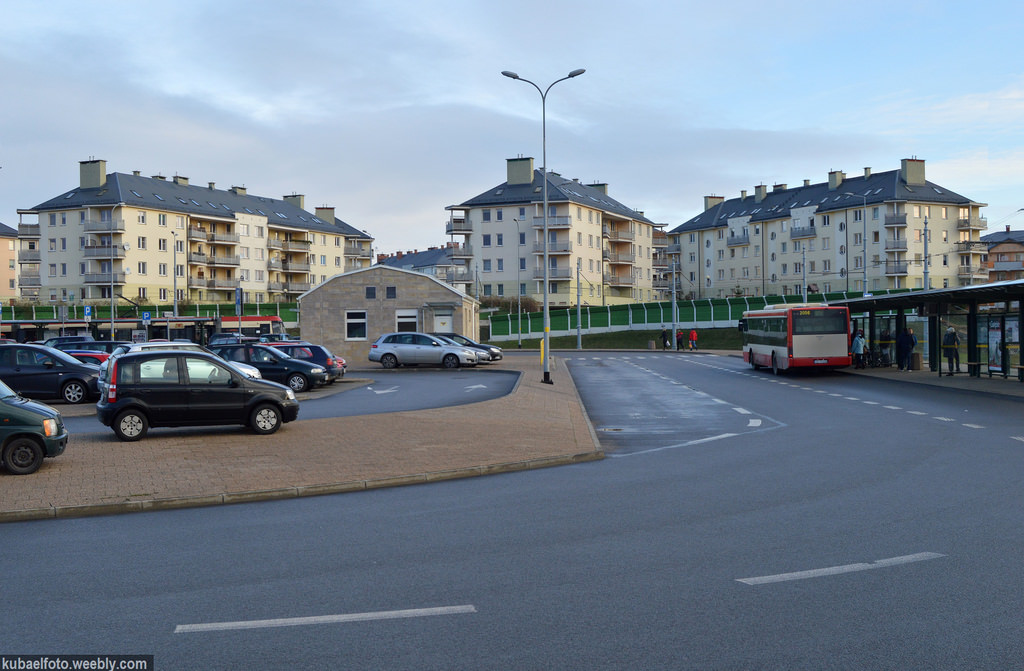
\includegraphics[width=1\linewidth]{Grunwaldzki/3}\\
		\footnotesize{źródło: Gisterek I., wykład wykład w formie elektronicznej, Zakład Infrastruktury Transportu Szynowego, Politechnika Wrocławska, \url{http://www.zm.org.pl/download/prezentacje/0909-gisterek_pwroc.pdf} \cite{grunwaldzki2}}
		\label{grunwaldzki3}
	\end{figure}	
	
	Przyjęcie rozwiązania w formie dużego skrzyżowania z węzłem znajdującym się na wyspie centralnej zapewniło przede wszystkim zebranie wszystkich rodzajów transportu w obręb jednego obszaru. Dzięki temu możliwa jest duża dowolność wyboru połączenia bez konieczności przemieszczania się przez skrzyżowanie. Odpowiednie formy transportu zostały pogrupowane w zależności od kierunku jazdy aby umożliwić pasażerom wybór najszybszego pojazdu. Przykładowo, tramwaje jadące w kierunku mostu Grunwaldzkiego (linie 0, 2, 4) wszystkie zatrzymują się na przystanku południowym. 
	
	Węzeł wyposażony jest w szerokie przejście podziemne z windami dla osób niepełnosprawnych. Problematyczny jest brak ramp i pochylni. Na powierzchni, przystanki posiadają ławki i zadaszenie w postaci wiat stalowych. Na terenie węzła znajdują się trzy biletomaty, wyświetlacze z aktualnymi kursami pojazdów oraz tablice z rozkładami jazdy. Nawierzchnia torowiska tramwajowego wykonana jest z kostki, która na stan obecny (maj 2018) jest w bardzo złym stanie (co widać na przykład na rysunku \ref{grunwaldzki5}. Wysokość torowiska to zaledwie kilka centymetrów poniżej poziomu chodnika przez co wsiadanie i wysiadanie z pojazdów jest uciążliwe dla pasażerów co pokazano na rysunku \ref{grunwaldzki6}. Poszczególne przystanki oddzielone są przejściami dla pieszych wyposażonymi w sygnalizację świetlną. 
	
	\begin{figure}[H]
		\centering
		\caption{Widok na przystanek północny}
		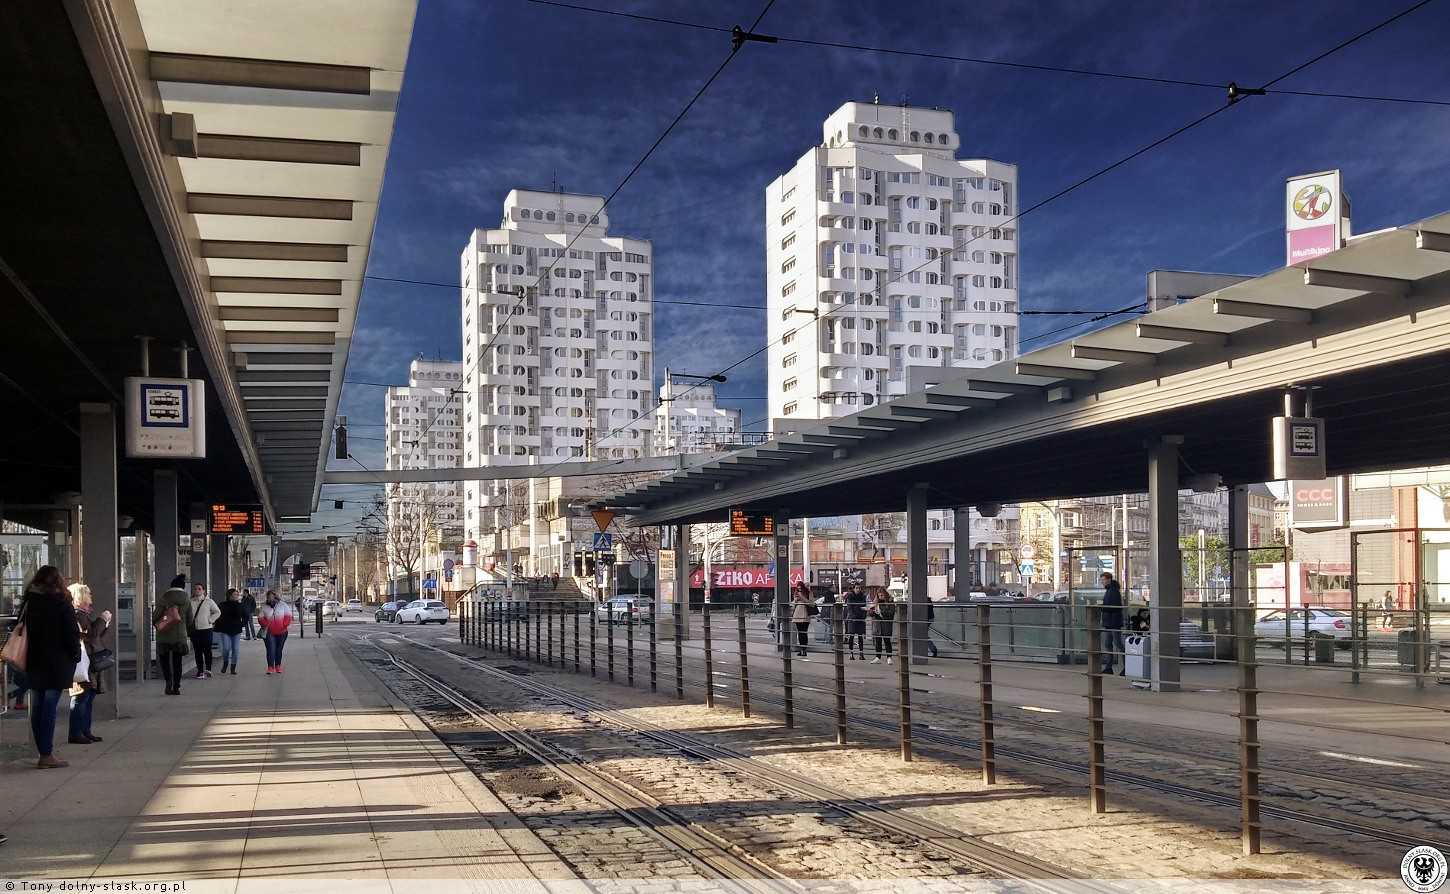
\includegraphics[width=0.8\linewidth]{Grunwaldzki/5}\\
		\footnotesize{źródło: Stowarzyszenie Wratislaviae Amici \url{https://dolny-slask.org.pl/3839663,Wroclaw,Wezel_przesiadkowy_Plac_Grunwaldzki.html}}
		\label{grunwaldzki5}
	\end{figure}	
	
		\begin{figure}[H]
		\centering
		\caption{Pasażerowie wsiadający do tramwaju}
		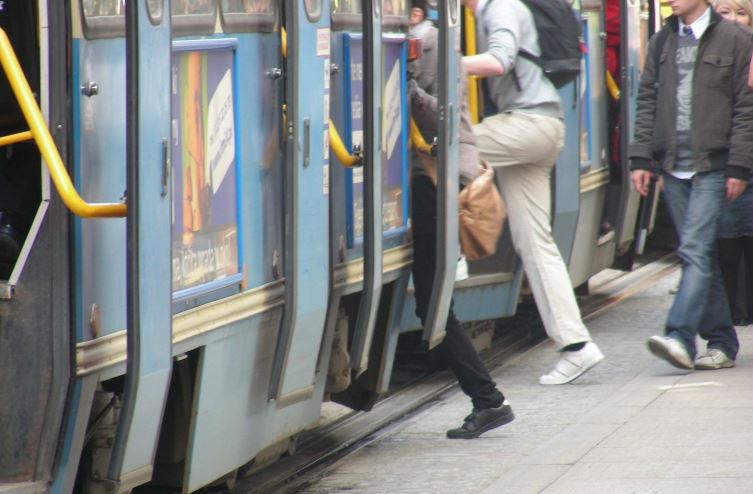
\includegraphics[width=0.8\linewidth]{Grunwaldzki/6}\\
		\footnotesize{źródło: Gisterek I., wykład wykład w formie elektronicznej, Zakład Infrastruktury Transportu Szynowego, Politechnika Wrocławska, \url{http://www.zm.org.pl/download/prezentacje/0909-gisterek_pwroc.pdf} \cite{grunwaldzki2}}
		\label{grunwaldzki6}
	\end{figure}	
	
	Przebudowa skrzyżowania w jeden zintegrowany węzeł tramwajowo-autobusowy zwiększyła komfort podróży pasażerów i cała inwestycja jest uznawana za udaną, jednak nie obyło się bez głosów krytyki. Przede wszystkim z powodu konieczności korzystania z przejść podziemnych aby dostać się do przystanków. Czas dojścia do docelowego przystanku wysłużył się w stosunku do tego przed przebudową. Dzisiejsze podejście zakłada priorytet pieszych nad pojazdami w centrach miast a nie sprowadzanie ruchu pieszego pod lub nad ziemię. Pierwotny projekt węzła zakładał dodatkowe przejścia dla pieszych umożliwiające dojście do przystanków z poziomu ulicy (co widać na początkowych wizualizacjach -- rysunek \ref{grunwaldzki2}), jednak zrezygnowano z nich przy oddawaniu węzła do użytku w 2008 roku pomimo wykonania odpowiedniej infrastruktury (obniżone krawężniki, ustawienie słupów pod sygnalizatory). Przejścia te pojawiły się dopiero w 2017 roku. Początkowy brak przejść dla pieszych wynikał jedynie z życzenia inwestora o czym mówił Marek Suchy z biura BBKS Projekt, które przygotowało projekt organizacji ruchu:
	\begin{quote}
	,,W naszym projekcie znalazły się przejścia dla pieszych, ale na życzenie inwestora zostały one usunięte. Ale nie ma technicznych przeszkód, żeby je nawet dzisiaj domalować. Moim zdaniem nie jest logiczne, by mieszkańcy musieli schodzić ponad 6 metrów w dół i później tyle samo w górę, by dostać się do peronu tramwajowego. Jest to niewygodne i czasochłonne.”
	\end{quote}
	
	Konieczność korzystania z przejścia podziemnego, które przez dostosowanie go do poziomu $-1$ galerii handlowej schodzi na głębokość aż 6 metrów, zmniejszała atrakcyjność węzła oraz była powodem dużej liczby nielegalnych przekroczeń jezdni, szczególnie pomiędzy wyspą centralną a przystankiem linii 1. Dużym problemem są także przejścia w obrębie węzła pomiędzy wyspami, których czas międzyzielony jest zbyt długi. W efekcie większość pieszych przekracza jezdnie podczas światła czerwonego -- na trzech z czerech przejść liczba niedozwolonych przejść wynosiła ponad 70\% co pokazano w tabeli \ref{grunwaldzki4} \cite{grunwaldzki3}. Zalecanym rozwiązaniem w takim przypadku byłoby zastosowanie sygnalizacji wzbudzanej przez pojazdy, gwarantując tym samym długi czas światła zielonego pieszym. 
	
		\begin{table}[H]
		\centering
		\caption{Warunki ruchu pieszego na przejściach w obrębie węzła przesiadkowego}
		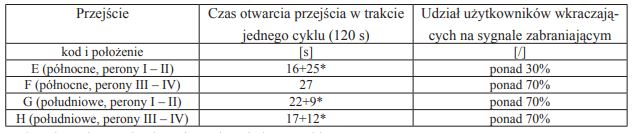
\includegraphics[width=1\linewidth]{Grunwaldzki/4}\\
		\footnotesize{źródło: Molecki B., \emph{Analiza ruchu pieszego w obrębie węzłów przesiadkowych na przykładzie placu Grunwaldzkiego we Wrocławiu}, Konferencja naukowo-techniczna ,,Zintegrowany system transportu miejskiego'', Wrocław, 27-28 maja 2010 \cite{grunwaldzki4}}
		\label{grunwaldzki4}
	\end{table}	

	Po wykonaniu przejść dla pieszych w obrębie węzła wzrosła jego atrakcyjność oraz liczba korzystających z niego pasażerów co pozwala pokazać silny związek między komfortem użytkowników a udziałem podróży. W miastach europejskich odchodzi się od prowadzenia tras pieszych w różnych poziomach niż domyślnie na poziomie chodnika. Pomimo rozbudowanego i wyposażonego w windy dla niepełnosprawnych przejścia podziemnego prowadzącego do wszystkich przystanków dopiero utworzenie wcześniej rozważanych przejść sprawiło, że węzeł ten podniósł jakość komunikacji w tym rejonie \cite{grunwaldzki3}. 
	
	


\clearpage
\begin{thebibliography}{99}

\bibitem{raport-vip}
	Bielecki P., \emph{Kształtowanie przyjaznych dla pieszych węzłów przesiadkowych w mieście}, Warszawska Inicjatywa Piesza, Zielone Mazowsze, listopad 2011.

\bibitem{standardy_wroclaw}
	Bocheńska-Niemiec A., Cebrat K., Kusowska K., Romanik A., Tyrka Ł., Walter E., Wiszniowski J., \emph{Wrocławskie standardy kształtowania przestrzeni miejskich przyjaznych pieszym}, Gmina Wrocław, maj 2017.

\bibitem{urbanistyka}
	Chmielewski J.M.,	\emph{Teoria urbanistyki w projektowaniu i planowaniu miast},	Oficyna Wydawnicza Politechniki Warszawskiej, Warszawa 2001.
	
\bibitem{czauderna}
	Czauderna T., \emph{Konstrukcje torów tramwajowych}, czasopismo ,,TTS Technika Transportu Szynowego'' nr 9/2004.
	
\bibitem{tp1}
	Czubiński R., \emph{Jak zaprojektować dobry węzeł przesiadkowy}, ,,Transport Publiczny'', 16 października 2010.
	
\bibitem{dijk}
	Dijk M., Montalvo C.,	\emph{Policy frames of Park-and-Ride in Europe},	,,Journal of Transport Geography'', nr 19/2011.
	
\bibitem{gazeta_gdansk}
	Dobaczewski J., Kraska A., Zomkomski S., \emph{ŁOŚ, czyli nowy Węzeł Integracyjny komunikacji miejskiej: Łostowice – Świętokrzyska}, Gazeta Metropolitalnego Związku Komunikacyjnego Zatoki Gdańskiej ,,Przystanek Metropolitarny'' nr 8, lipiec 2013, \url{http://www.zkmgdynia.pl/admin/__pliki__/290x400_x8_mzkzg_PrzystanekNr8%20internet.pdf}
	
\bibitem{grunwaldzki2}
	Gisterek I., wykład wykład w formie elektronicznej, Zakład Infrastruktury Transportu Szynowego, Politechnika Wrocławska, \url{http://www.zm.org.pl/download/prezentacje/0909-gisterek_pwroc.pdf}
	
\bibitem{mlociny4}
	Jackowski M., \emph{Węzeł komunikacyjny Młociny okiem pasażera}, II Warsztaty Forum LINK w Bydgoszczy, 21 września 2009.
	
\bibitem{standardy_chodnik}
	Józefowicz P., \emph{Katalog Standardów Nawierzchni Chodników dla Wrocławia}, Wrocław 2013.
	
\bibitem{kaszubowski}
	Kaszubowski D., \emph{Badanie jakości usług transportu zbiorowego na nowej trasie tramwajowej w dzielnicy Gdańsk Południe}, ,,Technika Transportu Szynowego'' nr 10/2013.
	
\bibitem{kazimierczyk}
	Kazimierczyk M., \emph{Koncepcja współczesnego węzła przesiadkowego -- praktyczny przykład rozwiązania}, Biuletyn Komunikacji Miejskiej IGKM, nr 136, maj 2015.
	
\bibitem{grunwaldzki1}
	Korycki T., Molecki B., Puchalski P., Wicher M., \emph{Historia i przebudowa węzła autobusowego przy placu Grunwaldzkim we Wrocławiu}, ,,Przewoźnicy i systemy transportowe'', nr 11/2008.
	
\bibitem{olsson}
	Lindström Olsson A.,	\emph{Factors that influence choice of travel mode in major urban areas. The attractiveness of Park \& Ride},
	Division of Transportation and Logistics, KTH Royal Institute of Technology 2003.
	
\bibitem{maciej_lada}
	Łada M., Birr K. \emph{Analiza zmian funkcjonowania transportu zbiorowego wynikających z budowy węzłów integracyjnych}, III Krakowska Ogólnopolska Konferencja Naukowa Transportu ,,KOKONAT'' Kraków, 21-22 kwietnia 2016.
	
\bibitem{makarova}
	Makarova I., Shubenkova K., Gabsalikhova L.,	\emph{Analysis of the city transport system's development strategy design pronciples with account of risks and specific features of spaial development},	czasopismo ,,Transport Problems'', Kazan Federal University, 12/2017.
	
\bibitem{makuch}
	Makuch J., wykład w formie elektronicznej, kurs Koleje Miejskie, Politechnika Wrocławska, \url{http://www.zits.pwr.wroc.pl/makuch/kmm_W1.pdf}
	
\bibitem{makuch2}
	Makuch J., \emph{Projektowanie przystanków tramwajowych dla bezpieczeństwa i wygody pasażerów}, X Konferencja Naukowo-Techniczna ,,Drogi Kolejowe '99'' Spała, 13-15 października 1999.

\bibitem{projektowanie_obiektow_motoryzacyjnych}
	Mikoś-Rytel W., Biedrońska J., Figaszewski J., Kozak K., Lisik A.,	\emph{Projektowanie obiektów motoryzacyjnych},	Wydawnictwo Politechniki Śląskiej, Gliwice 2008.
	
\bibitem{grunwaldzki4}
	Molecki B., \emph{Analiza ruchu pieszego w obrębie węzłów przesiadkowych na przykładzie placu Grunwaldzkiego we Wrocławiu}, Konferencja naukowo-techniczna ,,Zintegrowany system transportu miejskiego'', Wrocław, 27-28 maja 2010.
	
\bibitem{opracowanie_gdansk}
	Mordak R., WYG International Sp. z o.o., \emph{Studium wykonalności dla zadań inwestycyjnych i modernizacyjnych przewidzianych do realizacji w latach 2008-2011}, Gdański Projekt Komunikacji Miejskiej etap IIIa, Warszawa, listopad 2008.
	
\bibitem{oleksiewicz}
	Oleksiewicz W., Żurawski S., \emph{Drogi szynowe, podstawy projektowania linii i węzłów tramwajowych}, Zakład Inżynierii Komunikacyjnej Politechniki Warszawskiej, Warszawa 2004.
	
\bibitem{metodyka2}
	Olszewski P., Krukowska H., Krukowski P., \emph{Jak oceniać projektowane lub funkcjonujące węzły przesiadkowe?}, ,,Biuletyn Komunikacji Miejskiej'' nr 143, 2017.
	
\bibitem{metodyka}
	Olszewski P., Krukowska H., Krukowski P.,	\emph{Metodyka oceny wskaźnikowej węzłów przesiadkowych transportu publicznego},
	 ,,Transport miejski i regionalny'', 	czerwiec 2014.
	 
\bibitem{mlociny1}
	Pudło J., \emph{Węzeł Metro Młociny -- lokalizacja i znaczenie}, InfoBus, 14 lipca 2013, \url{http://www.infobus.pl/wezel-metro-mlociny-lokalizacja-i-znaczenie_more_44933.html}
	 
\bibitem{rybczynska}
	Rybczyńska M.
	\emph{System strategicznych parkingów "Park and Ride"},
	\url{http://www.transport.um.warszawa.pl/transport-publiczny/system-strategicznych-parking-w-parkuj-i-jed}
	
\bibitem{tory_tramwajowe}
	Rychlewski J., Firlik B., Straszewski W., \emph{Wytyczne projektowania torów tramwajowych a obecnie używany tabor tramwajowy}, Archiwum Instytutu Inżynierii Lądowej nr 25, 2017. 
	 
\bibitem{spillar}
	Spillar R.J.,	\emph{Park-and-ride planning and design guidelines},	Parsons Brinckerhoff Inc. 1997.
	
\bibitem{rps}
	Stacey R.,
	\emph{The effectiveness and sustainability of Park and Ride},
	12 czerwca 2009
	 
\bibitem{stanko}
	Stańko K.,	\emph{Przegląd i charakterystyka systemów parkingowych}, czasopismo ,,Mechanika'', 2012.
	
\bibitem{szarata2}
	Szarata A.,
	\emph{Analiza wielkości parkingów Park and Ride zlokalizowanych w obszarach metropolitarnych}, czasopismo ,,Budownictwo i architektura'', kwiecień 2014.
	
\bibitem{szarata}
	Szarata A.	\emph{Ocena efektywności funkcjonalnej parkingów przesiadkowych (P+R)},	praca doktorska, Politechnika Krakowska, październik 2005.
	
\bibitem{prawo-lewisa}
	Szymalski W.,	\emph{Prawo Lewisa-Mogridge’a w Warszawie - wprowadzenie}, styczeń 2012,
	\url{http://www.zm.org.pl/?a=lewis-mogridge-14-00_wprowadzenie}
	
\bibitem{standardy_szwajcarskie}
	Szymalski W., \emph{Standardy szwajcarskie dla węzłów przesiadkowych}, czasopismo ,,Transport'', 14 marca 2018.
	
\bibitem{guide}
	Terzis G.,	\emph{GUIDE: group for urban interchanges development and evaluation},	marzec 2018.
	
\bibitem{mlociny2}
	Urbanowicz W., \emph{Warszawa: Jak poprawić węzeł? ZTM ,,ulepszy'' Młociny}, 14 marca 2016, Transport Publiczny, \url{http://www.transport-publiczny.pl/wiadomosci/jak-poprawic-wezel-ztm-ulepszy-mlociny-51577.html}
	
\bibitem{young}
	Young A., \emph{Manual for Streets. London.}, Thomas Telford Publishing, 2007.
	
\bibitem{zaluski}
	Załuski D., \emph{Zintegrowane węzły przesiadkowe przy małych dworcach kolejowych}, 
	,,TTS Technika Transportu Szynowego'' str. 62--68, nr 21, 2014.
	
\textbf{RAPORTY:}

\bibitem{florida}
	Florida Department of Transportation,	\emph{State Park-and-Ride guide}, czerwiec 2012
	
\bibitem{gothenburg}
	Goteborgs Stad,
	\emph{Fysisk planering för kollektivtrafik (Fizyczne planowanie transportu zbiorowego)},
	raport nr 1/2004.	
	
\bibitem{icaen}
	Katalońska Grupa ds. Efektywności Energii. Kataloński Instytut Energii,
	\emph{White Book of the Sustainable Mobility in the early XXI century}.
	
\bibitem{eurotest}
	RACC foundation, MoviNews:
	\emph{Park \& Ride; State of the Art in Europe}. ,,EuroTest'' nr 9 -- marzec/kwiecień 2009.
	
\bibitem{grunwaldzki3}
	Stowarzyszenie ,,Akcja miasto'', \emph{Raport o ruchu pieszych we Wrocławiu}, 2015.
	
\bibitem{guidelines_washington}
	Washington Metropolitan Area Transit Authority, \emph{Guidelines for station site and access planning}, Sierpień 2005.
	
\bibitem{poznan}
	Zespół Blue Ocean Business consulting ds. transportu publicznego,
	\emph{Koncepcja budowy funkcjonalnych węzłów przesiadkowych PKM w kierunku zwiększenia ich dostępności oraz oferowania usług komplementarnych do komunikacji publicznej},
	Lipiec 2015.
	
	\clearpage
\textbf{NORMY I ROZPORZĄDZENIA:}

\bibitem{wytyczne_ulice}
	Generalna Dyrekcja Dróg Publicznych, \emph{Wytyczne projektowania ulic}, Instytut Badawczy Dróg i Mostów, Warszawa, 1992.
	
\bibitem{knd_podatne}
	Generalna Dyrekcja Dróg Krajowych i Autostrad, \emph{Katalog typowych konstrukcji nawierzchni podatnych i półsztywnych}, opracowanie Katedry Inżynierii Drogowej Politechniki Gdańskiej, Gdańsk 2014.
	
\bibitem{knd_sztywne}
	Generalna Dyrekcja Dróg Krajowych i Autostrad, \emph{Katalog typowych konstrukcji nawierzchni sztywnych}, opracowanie Katedry Dróg i Lotnisk Politechniki Wrocławskiej, Wrocław 2014.
	
\bibitem{ustawa_transport}
	Ustawa z dnia 16 grudnia 2010 r. o publicznym transporcie zbiorowym: Dz.U. 2011 nr 5 poz. 13.
	
\bibitem{rozporzadzenie_drogi}
	Rozporządzenie Ministra Transportu i Gospodarki Morskiej z dnia 2 marca 1999 r. 
	w sprawie warunków technicznych, jakim powinny odpowiadać drogi publiczne i ich usytuowanie (Dz. U. z 1999r. nr 43, poz. 430).
	
\bibitem{warunki_techniczne}
	Rozporządzenie Ministra Infrastruktury z dnia 12 kwietnia 2002 r. 
	w sprawie warunków technicznych, jakim powinny odpowiadać budynki i ich usytuowanie (Dz. U. z 2015r. poz. 1422)
	

	
\textbf{STRONY INTERNETOWE:}

\bibitem{biezanow1}
	Gazeta Wyborcza Kraków, \emph{Weźże zaparkuj i jedź tramwajem. Park\& Ride już w Bieżanowie}, \url{http://krakow.wyborcza.pl/krakow/7,44425,22901021,wezze-zaparkuj-i-jedz-tramwajem-park-ride-juz-w-biezanowie.html}
	
\bibitem{oltaszyn}
	Gołębiewska M., \emph{Trasa tramwajowa na Ołtaszyn będzie dłuższa? Jest szansa, że tramwaj obsłuży też Wysoką}, Serwis TuWrocław,\url{https://www.tuwroclaw.com/wiadomosci,trasa-tramwajowa-na-oltaszyn-bedzie-dluzsza-jest-szansa-ze-tramwaj-obsluzy-tez-wysoka,wia5-3273-38956.html}
	
\bibitem{biezanow4}
	Magiczny Kraków, \emph{Parking P+R w Nowym Bieżanowie otwarty}, 15 stycznia 2018, \url{http://krakow.pl/aktualnosci/216797,1912,komunikat,parking_p+r_w_nowym_biezanowie_otwarty.html}
	
\bibitem{biezanow2}
	Miejska Infrastruktura Kraków, \emph{P\& R Bieżanów}, \url{http://mi.krakow.pl/parkingi/inwestycja-biezanow}
	
\bibitem{mlociny3}
	Oficjalny serwis Metra Warszawskiego, \emph{Budowa tunelu B23 i stacji A23 Młociny wraz z węzłem komunikacyjnym}, \url{http://www.metro.waw.pl/budowa-tunelu-b23-i-stacji-a23-mlociny-wraz-z-wezlem-komunikacyjnym}

\bibitem{oxford}
		Oxford Mail, \emph{How Oxford led the way to create Park and Rides},	6 grudnia 2013,
	\url{http://www.oxfordmail.co.uk/news/10859209.How_Oxford_led_the_way_to_create_Park_and_Rides/}
	
\bibitem{oxford2}
	Oxfordshire county council:
	\url{https://www.oxfordshire.gov.uk/cms/public-site/park-and-ride}
	
\bibitem{portal_gdansk}
	Portal Miasta Gdańska, inwestycje miejskie, \url{http://www.gdansk.pl/inwestycje-miejskie/Gdanski-Projekt-Komunikacji-Miejskiej-etap-III-A,a,17762}
	
\bibitem{tomtom}
	TomTom Traffic Index 2017.
	\url{https://www.tomtom.com/en_gb/trafficindex/}
	
\bibitem{biezanow3}
	Wiadomości nasze-miasto.pl Kraków, \emph{Parking Park\& Ride w Bieżanowie}, 2 lipca 2017, \url{http://krakow.naszemiasto.pl/artykul/parking-park-ride-w-biezanowie-wizualizacje,3440403,art,t,id,tm.html}
	

	
	
	
	
	
	
	

	

	

	



	

	

	

	

	

	

	

	

	

	

	

	

	

	

	

	
	
\end{thebibliography}
	


\end{document}
